\documentclass{article}
\usepackage{allan}
\usepackage{lastpage}
\usepackage{algorithmic}
\usepackage{algorithm}
\setlength{\headheight}{70pt}

\newcommand{\itembf}{\item \textbf}
\newcommand{\violetbf}[1]{\textcolor{violet}{\textbf #1}}
% \renewcommand{\baselinestretch}{1.2}


\lhead{
    \parbox{5cm}{
        \begin{center}
            Problem Chosen \\[0.2cm]
            \textbf{\Huge{A}}
        \end{center}
    }
}
\chead{
    \parbox{5cm}{
        \textbf{
            \begin{center}
                2022 \\
                MCM \\
                Summary Sheet
            \end{center}
        }
    }
}
\rhead{
    \parbox{5cm}{
        \begin{center}
            Team Control Number \\[0.2cm]
            \textbf{\Huge{2226594}}
        \end{center}
    }
}
\cfoot{}

\begin{document}
	\normalfont\fontfamily{qpl}\selectfont
    \begin{center}
        \textbf{\large Summary}

    \end{center}

	Under this problem, we've constructed a series of accurate models which both give the pattern of physical and physiological patterns of different cyclists during a time trial, and plausible suggestions to the athletes participating in different types of competitions. In the essay, instead of answering the questions by sequence, we've chosen a more natural narrative order which best displays the development of the models.

	In model A, we developed a differential model using motional, meteorological, and thermodynamic physics. After that, we separated the whole course into finite 'series' (parts that have similar physical attributes) of courses and performed our model on each individual 'series' based on recursion (initial values depend on the previous 'series'). In the end, we got the analytical solutions to almost all of the variables and those, after being plotted, fit well with the real-time data. At last, we used advanced mathematical tools to help scheme the distribution of energy, power, and velocity. By fitting our model on a self-designed course, we found that the cyclist's optimal strategy is to save energy (cycling purely with inertia) during the downhill slopes and find a compromising point between dashing with full force and maintaing high speed with minimum energy during the uphill slopes.

	In model B, we took into consideration that the 'splicing' action of 'series' appears to be less accurate with real-life courses. In order to make sure that our model works more accurately with the two major time-trials in the world, we rendered the discrete part of it into continuous differential equations. What's more, in model B, we also considered various psychological and physiological factors, including but not limited to the 'fatigue index' and the 'capabilities' of a specific athlete, which allows us to quantify an individual cyclist with a vector. Also, with the aid of Q-Learning algorithm on a multi-dimensional domain, our model eventually becomes dynamic.

	In model C, we focused on the team time trials (TTTs) with six participants. We formulate a plan which can rank the cyclists based on their physical conditions and calculate their benefit pattern when different people become the leader. Then we compare two kinds of leader exchanging and find out the best strategy. The model extend the participants, which enables us to apply it to any kinds of time trial, regardless of its type.

	As relevant constants that appear in our models are not always accessible on the Internet, we adopted the method of fitting data into our model, which derived rather reasonable results. To ahieve this, the neural networks of parameters is also employed with datasets of cyclists' performances from the Internet.

	Another part of our model with deep insight is that, instead of attempting to establish a universal model which is able to effectively cope with all types of scenarios, we developed two models (Model A \& B) which respectively excels in patterns with regular slopes and those with irregular ones. These two combined, therefore, actually results in a even more accurate model with computational convenience, accuracy and reality.



	% real document begins

    %%%%%%%%%%%%%%%%%%%%%%%%%%%%%%%%%%%%%%%%%%%%%%%%%%%%%%%%%%%%%%%%
    \clearpage
    \pagenumbering{arabic}
    \newpage
    \pagestyle{empty}
    \setlength{\headheight}{12pt}
    \renewcommand{\headrulewidth}{0.5pt}
    % \renewcommand{\headrulewidth}{5cm}
    \renewcommand{\footrulewidth}{0.0pt}
    \pagestyle{fancy}
    \lhead{Team \#2226594}
    \chead{Power Profile of a Cyclist}
    \rhead{Page \thepage\ of \pageref{LastPage}}
    \cfoot{}
    \lfoot{}
    \rfoot{}

    %%%%%%%%%%%%%%%%%%%%%%%%%%%%%%%%%%%%%%%%%%%%%%%%%%%%%%%%%%%%%%%%
    \clearpage
    \thispagestyle{empty}
    \tableofcontents
    \newpage
    \pagestyle{fancy}
    \setcounter{page}{1}

	\newpage
	\section{Introduction}
		\subsection{Background}
		Individual time trial is a common type of bicycle road race and has gained popularity in recent years. In individual time trials, individuals will manage to complete their journey on a fixed trial course all by themselves in the shortest possible time and the one that uses the minimum of time seals the victory.

		In cycling activities, each cyclist has a power curve which indicates the maximum power the rider can maintain in the races. Also, given a rider's power curve, cyclists must find the best way to minimize their power usage and maximize their recovering rate. In addition, there are many kinds of individual riders. Common types are time trial specialists, climbers, sprinters, rouleurs and puncheurs. They will act differently when facing various terrains and difficulties. Time trial specialists are good at solving every kinds of problems. The climbers can easily pass the long slopes while puncheurs perform well when facing cliffy slopes. Rouleurs can make good decisions based on different routes. Sprinters have strong explosive force. We will analyze their actions in the following passage.

		Moreover, the trial course plays a vital role in the game. It will determine how the cyclists spend their energy and control their speed. It has to be mentioned that all the riders will ride a same course. In games, the condition of trials mostly depends on the type of game and what kind of event it is.
		\subsection{Problem Restatement}
		To make sure that the riders can achieve their best score by using the best strategy (including when to get energy supply and recover) according  to their body condition, we need to find out the relationship between these factors. Therefore, our work is divided into 4 parts:
		\begin{itemize}
			\item  Analyze the power profile of two types if riders given their riding type.
			\item  Build a model calculating their power profile and find out the result when it is applied to different trial courses and various weather conditions. Find out how sensitive the model is.
			\item  Give suggestions to riders and their instructors generally on key turning points after determining how sensitive the model is.
			\item  Extend model so that it can be applied to conditions where a team will take part in a time trial.
		\end{itemize}
		\subsection{General Assumptions}
		\begin{enumerate}
			\item  \textbf{All the roads have the same rolling friction factors.}

					To help cyclists achieve better grades and prevent them from serious danger, race organizers usually build artificial tracks. Therefore we can assume that the material of tracks is the same, which means the rolling friction factor of the road is the same.
			\item  \textbf{All the riders know the terrain of the course and can make their decisions.}

					In most cases, riders are informed of the road condition far earlier than the race actually begins. In addition, knowing this in our model can avoid unnecessary calculations.
			\item  \textbf{The intake of metabolic energy can be stored.}

					If there is unconsumed energy during the riding process (e.g. breathing) , it will be stored. However, it will not exceed the maximum storage amount.
			\item  \textbf{Riders' cycling condition will not change when turning.}

					Road turns mainly contribute to the distraction of athletes. However, because turnings account for a timy proportion of the total time trial, the amount of energy consumed during this process can be ignored.
			\item \textbf{Riders consume no energy while going downhill.}

					Top cyclists usually tend to conserve their energy for uphill rides, which are critical to the overall result of the race. What's more, while riding downhill, riders need almost no energy to keep balance, so we won't consider any extra energy consumed when a rider goes downhill.
			\item \textbf{Every rider pre-expects a finishing time, which affects the type of strategy he/she adopts.}

					According to the second assumption, all the riders know the whole course. Therefore, we rightly assume that the participants all know there expected range of result before the race begins.

		\end{enumerate}

	\section{Model A: developing strategies for time trials}
		\subsection{Model Overview}
			In the first model, we will discuss the power curve of different types of cyclists. We will discuss the energy consumption of riders according their reactions towards different kinds of terrains and their body conditions. Considering basic energy cost such as breathing and processes of metabolism. We will calculate the power curve based on the maximum power a rider can reach in a certain time and how long he/she can maintain it. Finally, we will discuss the conditions where basic supplement is needed.
		\subsection{Notation}
			\begin{tabular}{|l|l|l|}
				\hline
				$t_\mathrm{exp}$&expected completing time&$\mathrm{s}$\\
				\hline
				$t_\mathrm{actual}$&actual completing time&$\mathrm{s}$\\
				\hline
				$t$&the time the game lasts for&$\mathrm{s}$\\
				\hline
				$P (\mathrm{w})$&power of a cyclist&W\\
				\hline
				$\tau(\mathrm{p})$&time which the rider last for at a constant power ($P (\mathrm{w})$)&$\mathrm{s}$\\
				\hline
				$m(t)$&the maximum power in the whole process&$\mathrm{W}$\\
				\hline
				$m( b )$&the maximum power of human body&$\mathrm{W}$\\
				\hline
				$\sigma$&speed of metabolism&$\mathrm{W}$\\
				\hline
				$ E _\mathrm{B}$&energy stored before the race&$\mathrm{J}$\\
				\hline
				$ E _\mathrm{S}$&energy supplied during the race&$\mathrm{J}$\\
				\hline
				$\tau( E _\mathrm{S})$&time wasted when recovering&$\mathrm{s}$\\
				\hline
				$ k $&power restriction index&/\\
				\hline
				$m$&weight of cyclist&$\mathrm{kg}$\\
				\hline
				$f$&air resistance&$\mathrm{N}$\\
				\hline
				$v$&speed of cyclist&m/s\\
				\hline
				$ C _ D $&air resistance index&/\\
				\hline
				$\rho_\mathrm{air}$&air density&\(\mathrm{kg/m}^3\)\\
				\hline
				$\mathrm{S}_\mathrm{body}$&cyclists' area exposed to air&$\mathrm{m}^2$\\
				\hline
				$ k _\mathrm{air}$&air condition index&/\\
				\hline
				$D$&distance&m\\
				\hline
				$I$&momentum gathered by wind&$\mathrm{N}$\\
				\hline
				$ E _\mathrm{total}$&the total energy stored before the race&$\mathrm{J}$\\
				\hline
				\(u\) & the rolling friction factor of the course & / \\
				\hline
				\(d_{\mathrm{strategy}}\left(\theta\right)\) & the changing point of strategy choice & \(\mathrm{m}\) \\
				\hline
			\end{tabular}
		\subsection{Calculating Energy Consumption}
			First, we need to consider the cyclist's energy source. We divide a rider's energy consumption into several parts. Considering human's basic physiological activities, energy spent by metabolism needs to be calculated. Therefore we use $\sigma$ to describe human body's speed of metabolism, which is a constant of value 41.5. Moreover, the rider's physical fitness determines his/her total energy before the race which is defined as $ E _\mathrm{total}$. Finally, cyclists can get energy before the race and energy supplied during the race through food consumption (which we define as $ E _\mathrm{B}$ and $ E _\mathrm{S}$).

			We use $P(t)$ to desribe the cyclist's power consumption pattern, $E(t)$ for remaining energy, and $v(t)$ for the velocity of each cyclist. All three functions change through time. However, many of the constants used in this model are not available on the Internet. Therefore, we chose the method of searching for more well-known data such as the speed of athlete, etc., and then fit these data with our model, which in turn derives reasonable factors which can be used to further our calculations.

			\subsubsection{developing strategies on vanilla cases}
			The record speed of time time trial cycling on plain ground is 36.6$\mathrm{m/s}$ \cite{time trial record}, which will later be used to decide relative constants.

			We define a \defword{series} by meaning of a finite continuous sequence of only uphill slopes or plain ground. According to \textbf{assumption 5}, we can abstract the ride into finite uphill/flat rides followed by downhill slopes, meaning that the whole 'series' of \defword{series} is an alternating combination of the two types. For the latter part, the functions can be calculeted independent of the strategies. Therefore, we repeat the calculations on each \defword{series}, and the following one can be calculated based on the previous one.

			When a cyclist takes part in a time trial, he/she needs to take some kind of strategy to make sure he/she makes a good performance. According to physical analysis, one of the best strategies is to use the greatest power at the beginning of the race, and then use a less power to maintain the speed he/she has accelerated to. In the final part of the race, where he/she no longer has energy, the inertia can take him/her to the ending point.

			Through a brief qualitative analysis, we can devide the senario into two parts:
			\begin{itemize}
				\item For a part that is short enough for the athlete to dash with full force (which means that there will still be energy left at the end of this period), we simply adopt this strategy because obviously this is the fastest possible strategy. However, for this type of strategy, we always have a maximum distance \(d_{\mathrm{strategy}}\left(\theta\right)\) beyond which we can no longer use this approach.


					Next, we will discuss the relationship between different variavbles. First, we do the force analysis on the cyclist and the bike as a whole:

					\begin{center}
						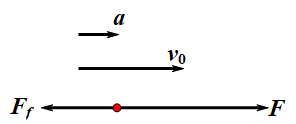
\includegraphics[height=2cm]{4.png}
						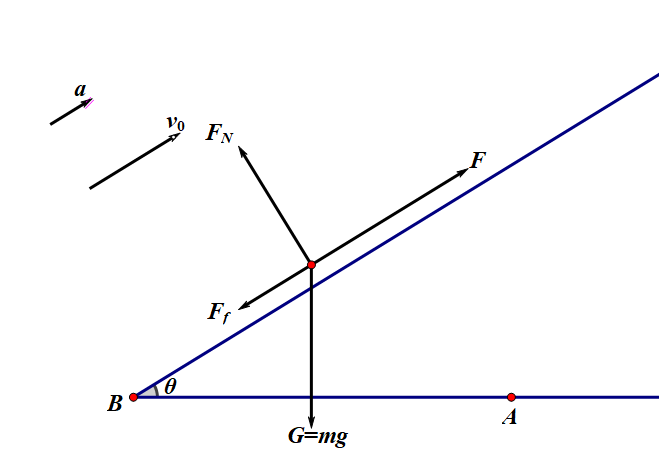
\includegraphics[width=5cm]{5.png}

						\small \textit{Fig. 1 and 2 A cyclist's condition on plain ground and uphill slopes}
					\end{center}

					Since the cyclists will race against each other at a quick speed, the air resistance ($f$) can't be neglected. According to basic physical rules, we can calculate \(f\) with the following formula:
					$$f=\dfrac{1}{2}  C _ D  \cdot \rho_\mathrm{air} S_\mathrm{body} v^2$$
					where \(C_D\) represents the area facing the wind. To be clear, let
					$$ k _\mathrm{air}=\dfrac{1}{2}  C _ D  \rho_\mathrm{air}$$
					therefore rewriting the previous equation, we have:
					$$f= k _\mathrm{air}\cdot v^2$$
					After searching related data from academic literature, we find out that $ C _ D =0.024$, $\rho_\mathrm{air}=1.293 \mathrm{kg/m}^3$ and $\mathrm{S}_\mathrm{body}=0.209 m^2$. Based on these data, we can indicate that $ k _\mathrm{air}\approx0.0032$.

					According to basic phycial rules (namely \textit{Newton's second law of motion}), we listed the formulae related to motion (\(v\left( t \right) ,a\left( t \right) ,D=s\left( t \right) \)) below (restrictions are also given based on initial set values):
					$$
					\begin{cases}
						\displaystyle
						D=\int^{t_\mathrm{actual}}_0 v(t)\cdot  D t\\
						m \cdot  a (t)=m \cdot v\dot(t)=F-f-mg\sin\left(\theta\right)=\dfrac{P (t)}{v}-\dfrac{1}{2} k_{\mathrm{air}} v^2-mg\sin\left(\theta\right)\\
						v(0)=0\\
						0\leq P (t)\leq m_ b\\
					\end{cases}
					$$

					As for the cyclist, the two variables that will alter his/her performance are mainly \(E(t)\) and \(P(t)\), which respectively indicates the remaining energy and current power at time \(t\).

					Referring to certain articles\cite{114514}, several constants are given below: we define $k$ as the index which describes the restriction of power.
					\[P \dot(t)=-\dfrac{1}{ k } P (t) \cdot \dfrac{1}{ E (t)}\]
					Which means, on a qualitative basis, means that the larger \(P(t)\) is (how hard he/she is riding), and the smaller \(E(t)\) is (how tired he/she is), the faster \(\dot{P(t)}\) will be (he/she will be exhausted more quickly).

					On the other hand, a formula is also needed to relate \(E(t)\) with the previously discussed motional variables. We notice that the derivative of \(E(t)\), or the instant power change, can be described as \(P_{\mathrm{intake}} - P_{\mathrm{output}}\). The second term can be calculated as \(\dot{E}_{\mathrm{output}}=F\cdot \dot{D\left( t \right)} =Fv\left( t \right) \). Therefore, we get the following formulae (restrictions are also given based on initial set values):
					$$
					\begin{cases}
						\displaystyle
						E \dot(t)=\sigma-\left(f+mg\sin\theta+\dfrac{mgu}{r_{\mathrm{wheel}}}\right)\cdot v(t) \\
						E (0)= E _\mathrm{total} \\
						E (t)\geq0,\, \forall\,0 \leq t \leq t_\mathrm{total} \\
					\end{cases}
					$$
					\(\Rightarrow E (t)=\left[\sigma-\left(f+mg\sin \theta +\dfrac{mgu}{r_{\mathrm{wheel}}} \right)\cdot v(t)\right]\cdot t+ E _\mathrm{total}\)

					We substitute the three equation sets above into one equation below:
					\[E (t)=-\dfrac{P (t)}{ k \cdot P \dot(t)}=-\dfrac{mv\ddot(t)+\dfrac{1}{2} k {v(t)}^3}{mv\dot(t)\cdot v(t)+v\dot(t)^2+\dfrac{3}{2} k {v(t)}^2}\]

					To increase reality and accuracy, we notice the fact that not all of the consumed energy can be converted into actual force. Therefore, we add a pre-factor \(\epsilon\) before the \(P_{\mathrm{output}}\). The factor will be calculated through comparations with real-life data. As mentioned before, we use world-record data to achieve this. (Notice that the formulae above also change with the emergece of \(\epsilon\))
					\[ -\dfrac{mv\ddot(t)+\dfrac{1}{2} k {v(t)}^3}{mv\dot(t)\cdot v(t)+v\dot(t)^2+\dfrac{3}{2} k {v(t)}^2} =  \left[\sigma-\epsilon\cdot\left(f+mg\sin \theta + \dfrac{mgu}{r_{\mathrm{wheel}}} \right)\cdot v(t)\right]\cdot t+ E _\mathrm{total}\]

					Out of brevity concerns, we let
					\[ \mathrm{A}=F_m-\dfrac{mgu}{\mathrm{r}_\mathrm{wheel}}-mg\sin \theta \]
					and then by solving the differential equation above, we can get the expression of \(v(t)\) as follows:

					\[v(t)=\dfrac{\sqrt{\mathrm{A}} \tan  h \left[\dfrac{\left(m C _1+t\right)\sqrt{\mathrm{A}k}}{m}\right]}{\sqrt{ k }}\]
					After solving the differential equation above and calculating the appropriate \(\epsilon\), we plot the velocity function \(v\left(t\right)\) as follows:

					\begin{center}
						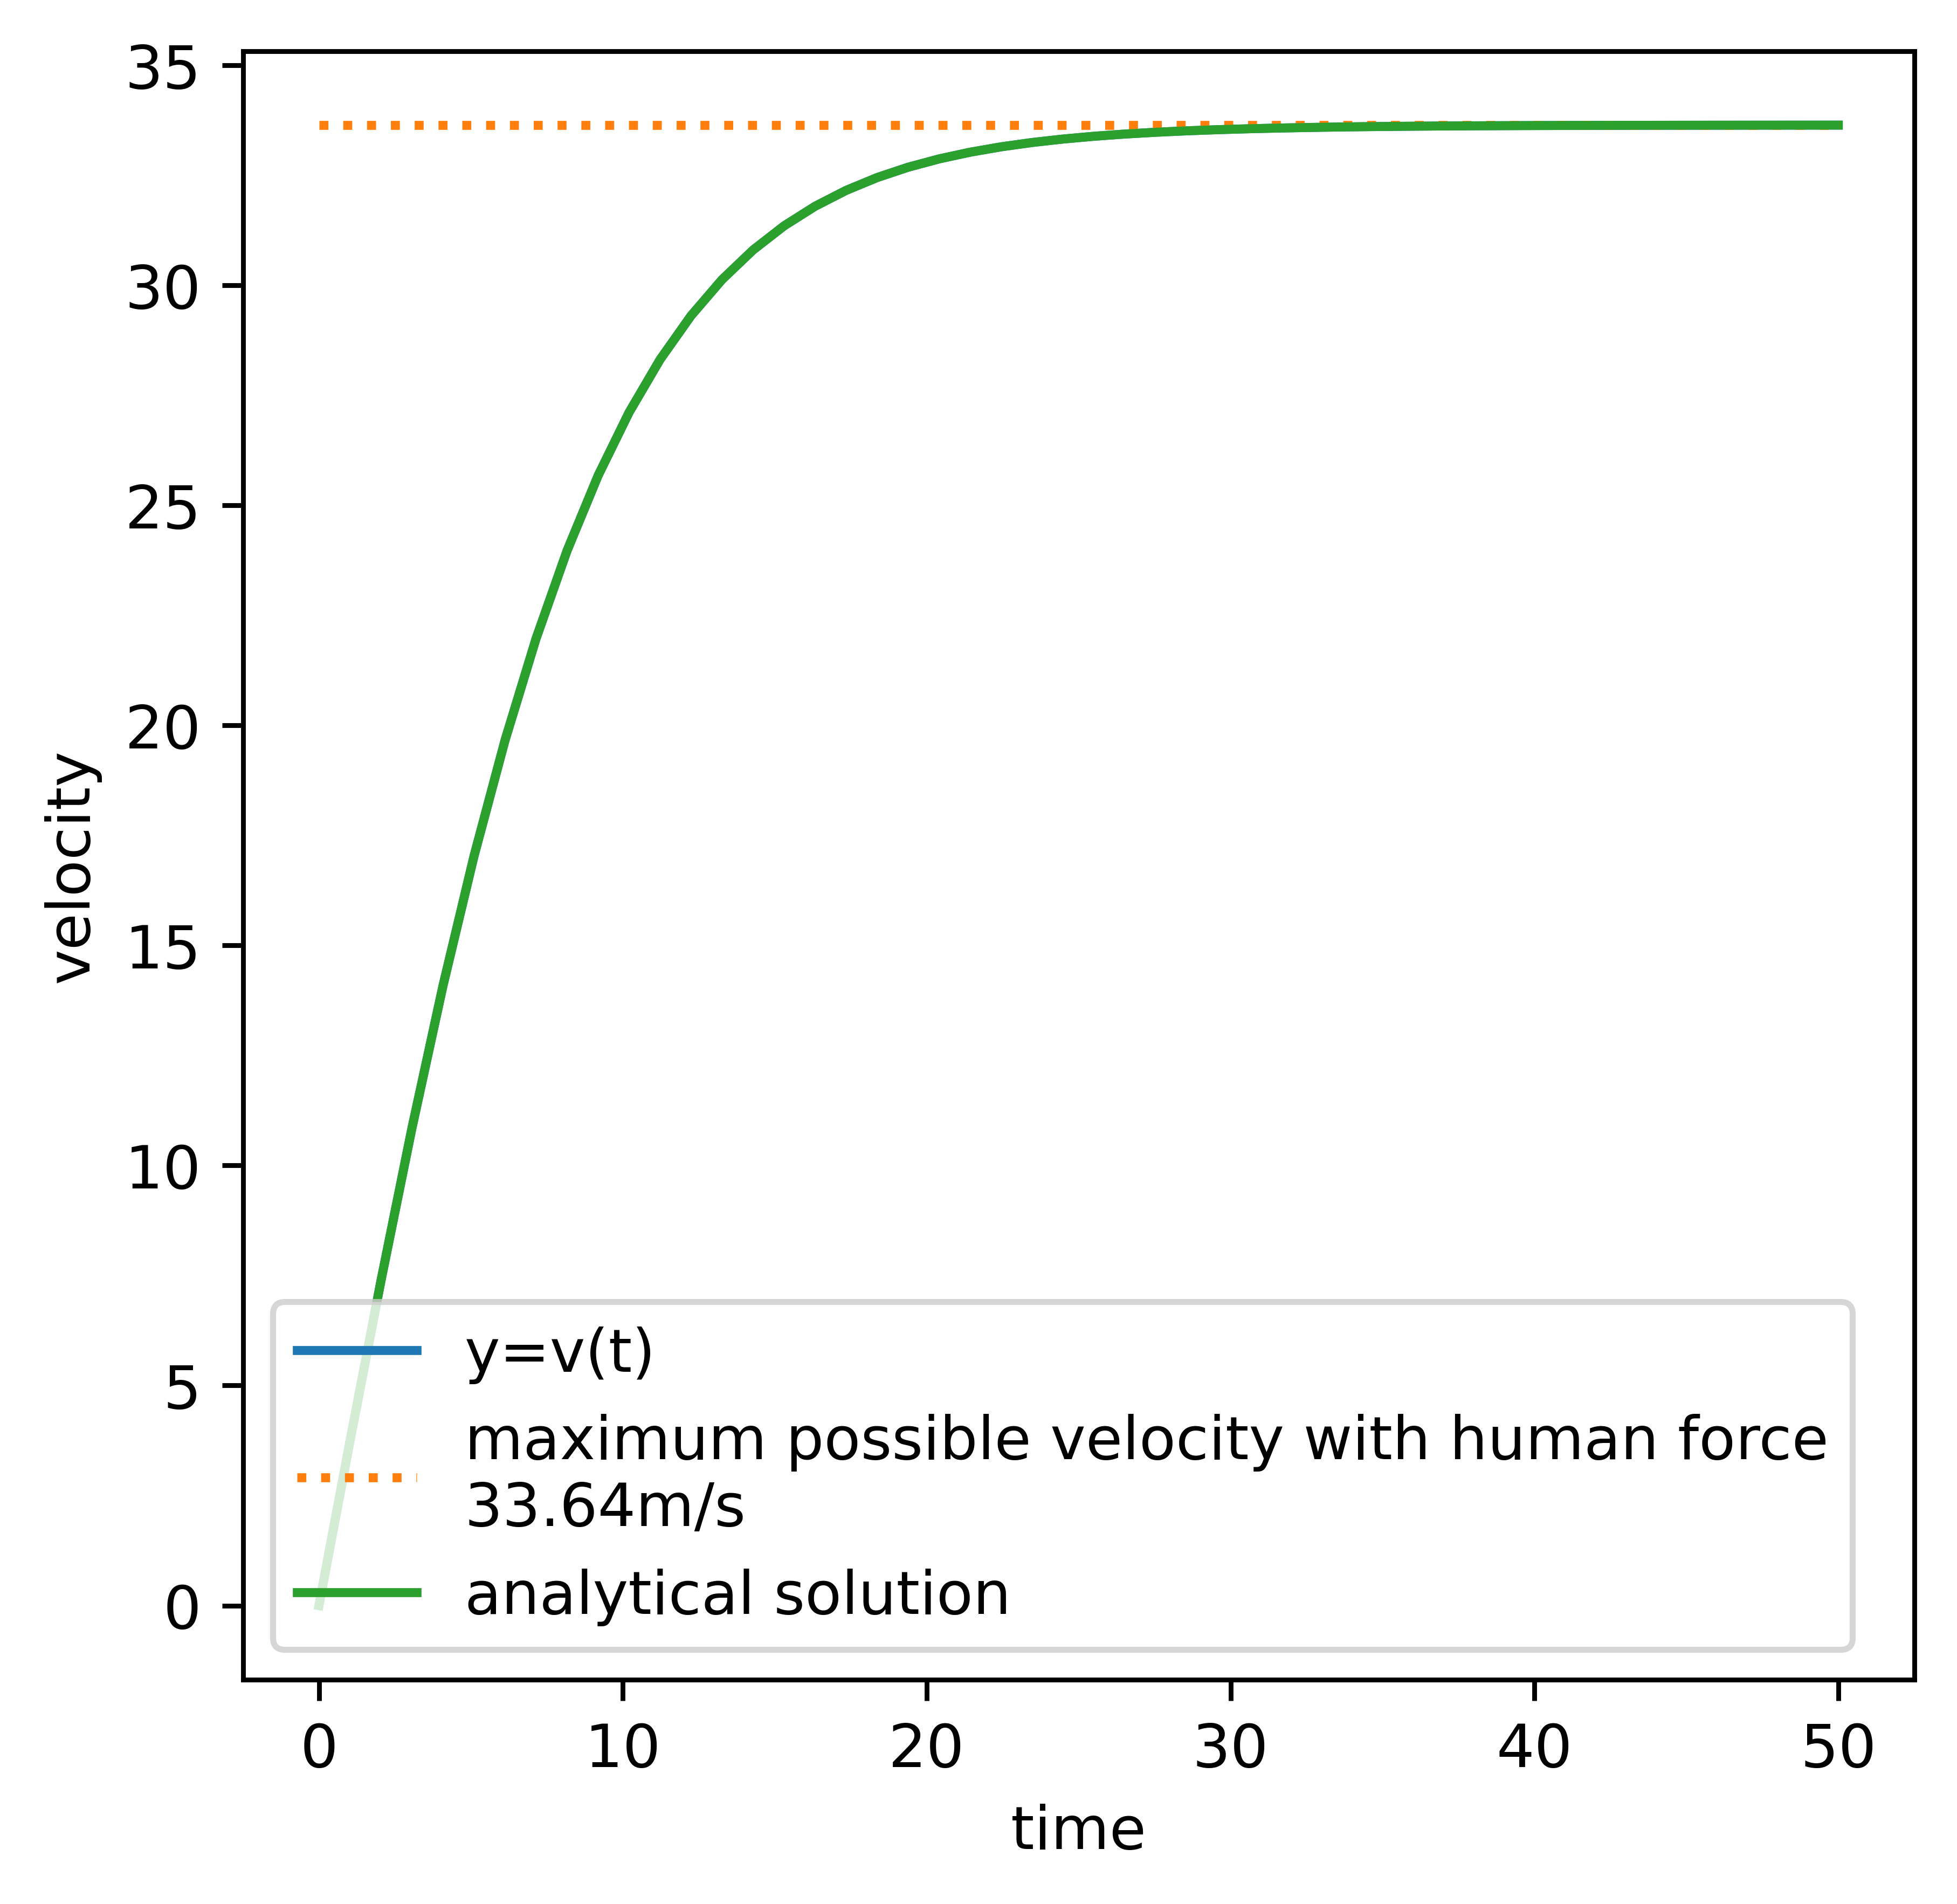
\includegraphics[height=6cm]{1.png}
						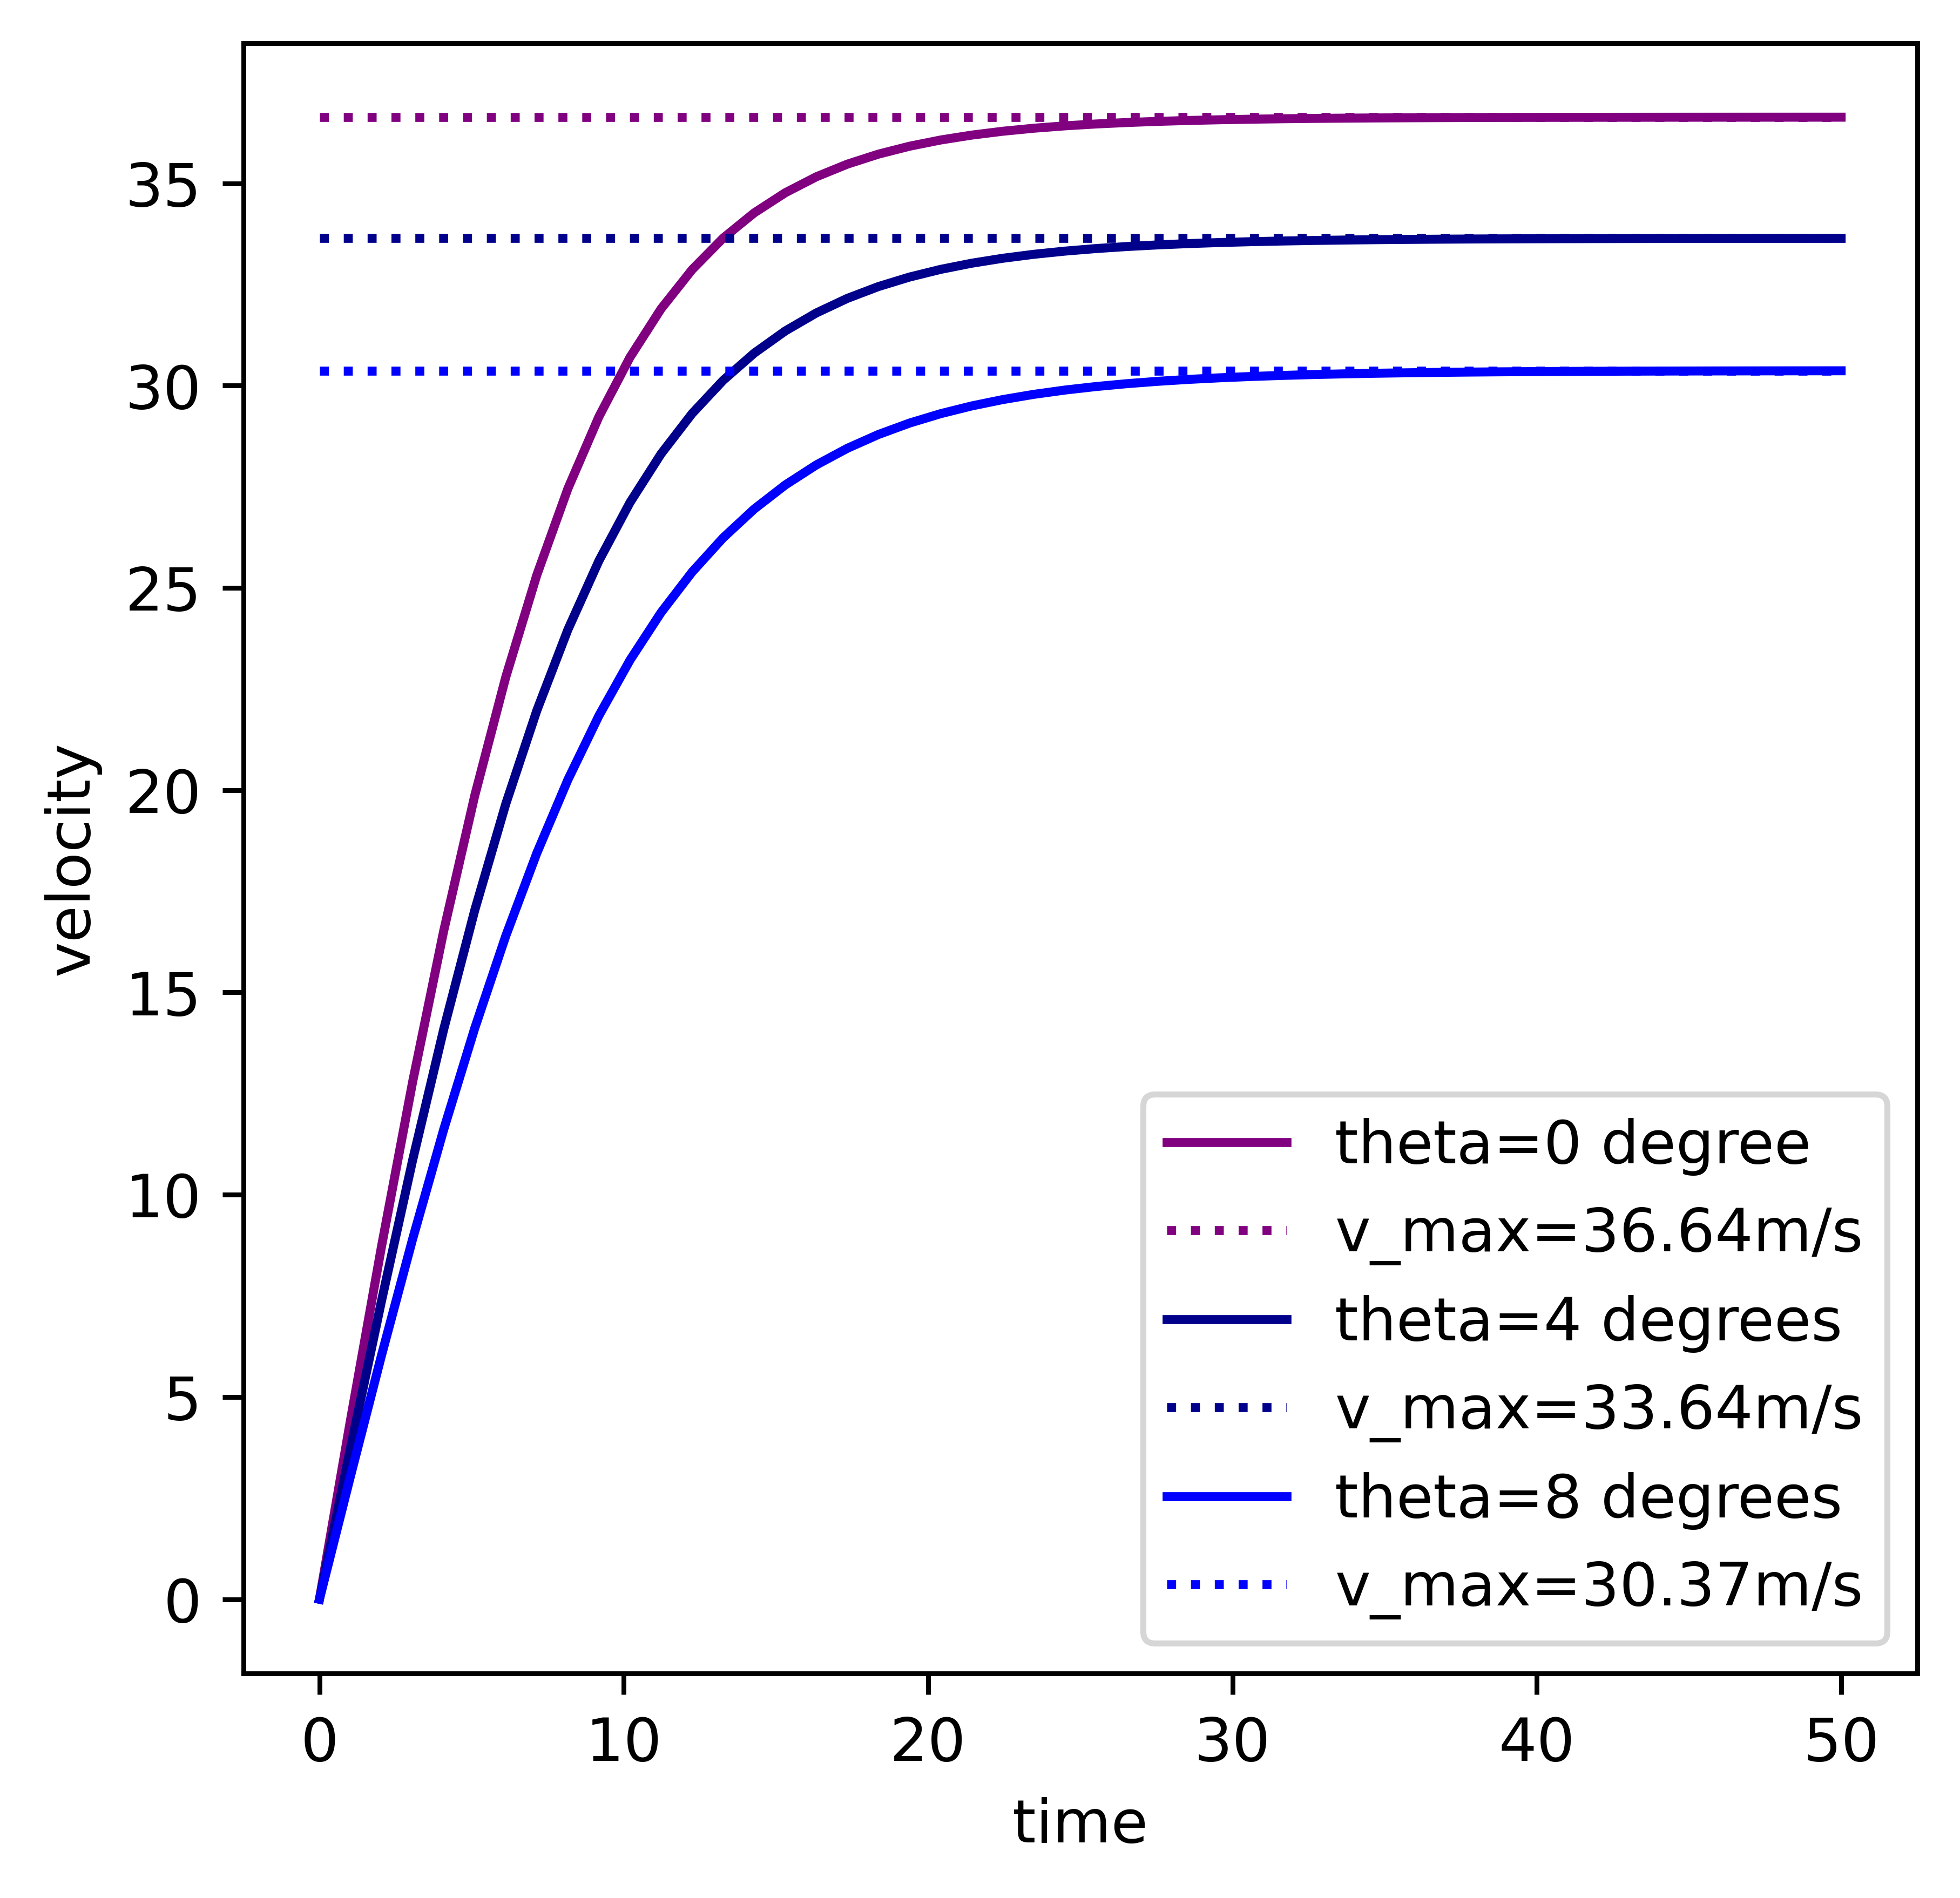
\includegraphics[height=6cm]{2.png}

						\small \textit{Fig. 4 and 5 Patterns of $v(t)$ on different slopes}
					\end{center}

					We also plot function \(E(t)\) as below:
					\begin{center}
						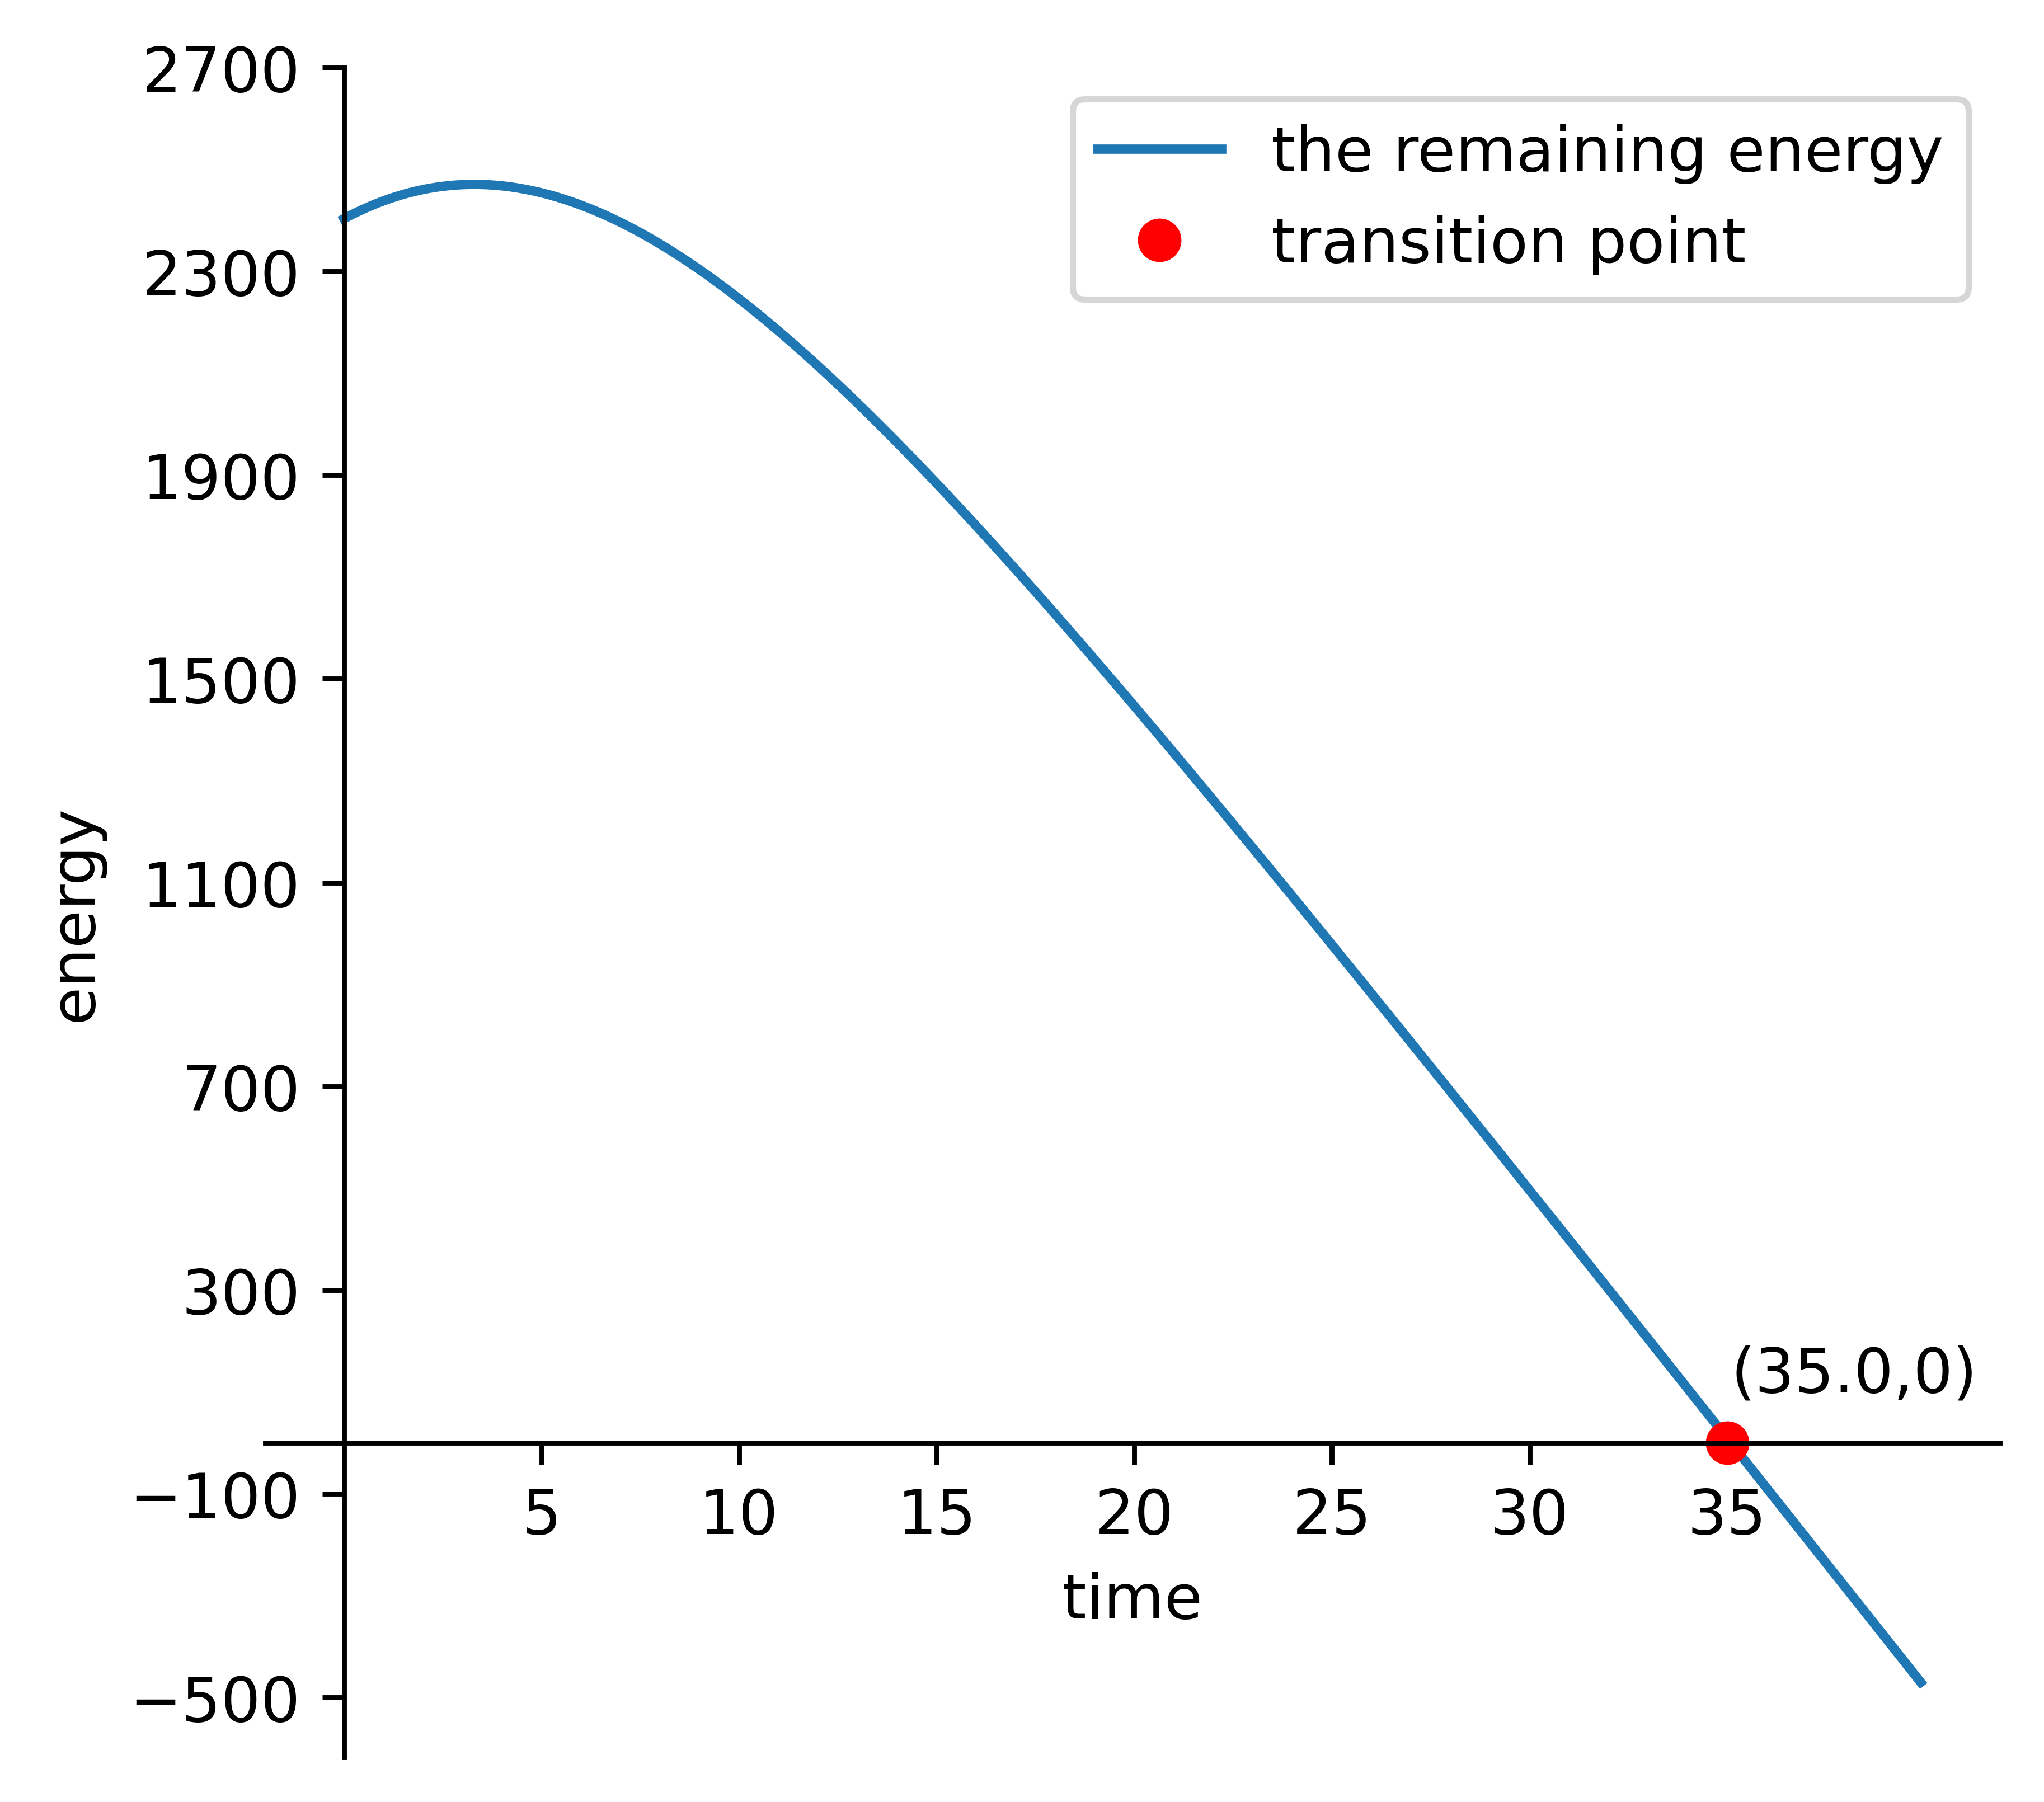
\includegraphics[height=5cm]{3.png}

						\small \textit{Fig. 6 Energy Pattern when dashing}
					\end{center}
					We can find that if a cyclist starts dashing, his/her remaining energy will have a sharp decline. The transition point \(\left(t_0,0\right)\) (the point where \(E(t) = 0\) represents the maximum time a rider can dash at full power before being exhausted. By observing the graph, we can find that \(t_0\) equals 35.0 $\mathrm{s}$. In addition, by integrating the velocity function, we can get the farthest that an athlete can go under this scenario:
					\[D_{\mathrm{first}\:\:\mathrm{phase}}=\int_0^{t_0}{v\left( t \right)  D t}\]
					,giving that the maximum dashing distance is 788.3$m$.

				\item For a part that is longer than that \(d_{\mathrm{strategy}}\left(\theta\right)\), we choose another strategy: at first, we use a certain amount of energy to \textit{push} the cyclist for a set period of time (which will be discussed later) before it enters the second phase, where the cyclist gradually depletes its energy till it reaches zero. In the end, the cyclist uses his/her remaining inertia to enter the next \defword{series} (downhill course).

					In the first accelerating part, we assume that it lasts for $t_1$ and the final speed it accelerates to is $v_1$. For the second part, we assume that it lasts for $t_2-t_1$, and obviously the speed of this part is stable at $v_1$. And according to our previous assumptions, the energy remaining at time $t_2$ should be zero. We should maximize the distance he/she covers in the whole period with the upwards conditions using calculus.
					\begin{center}
						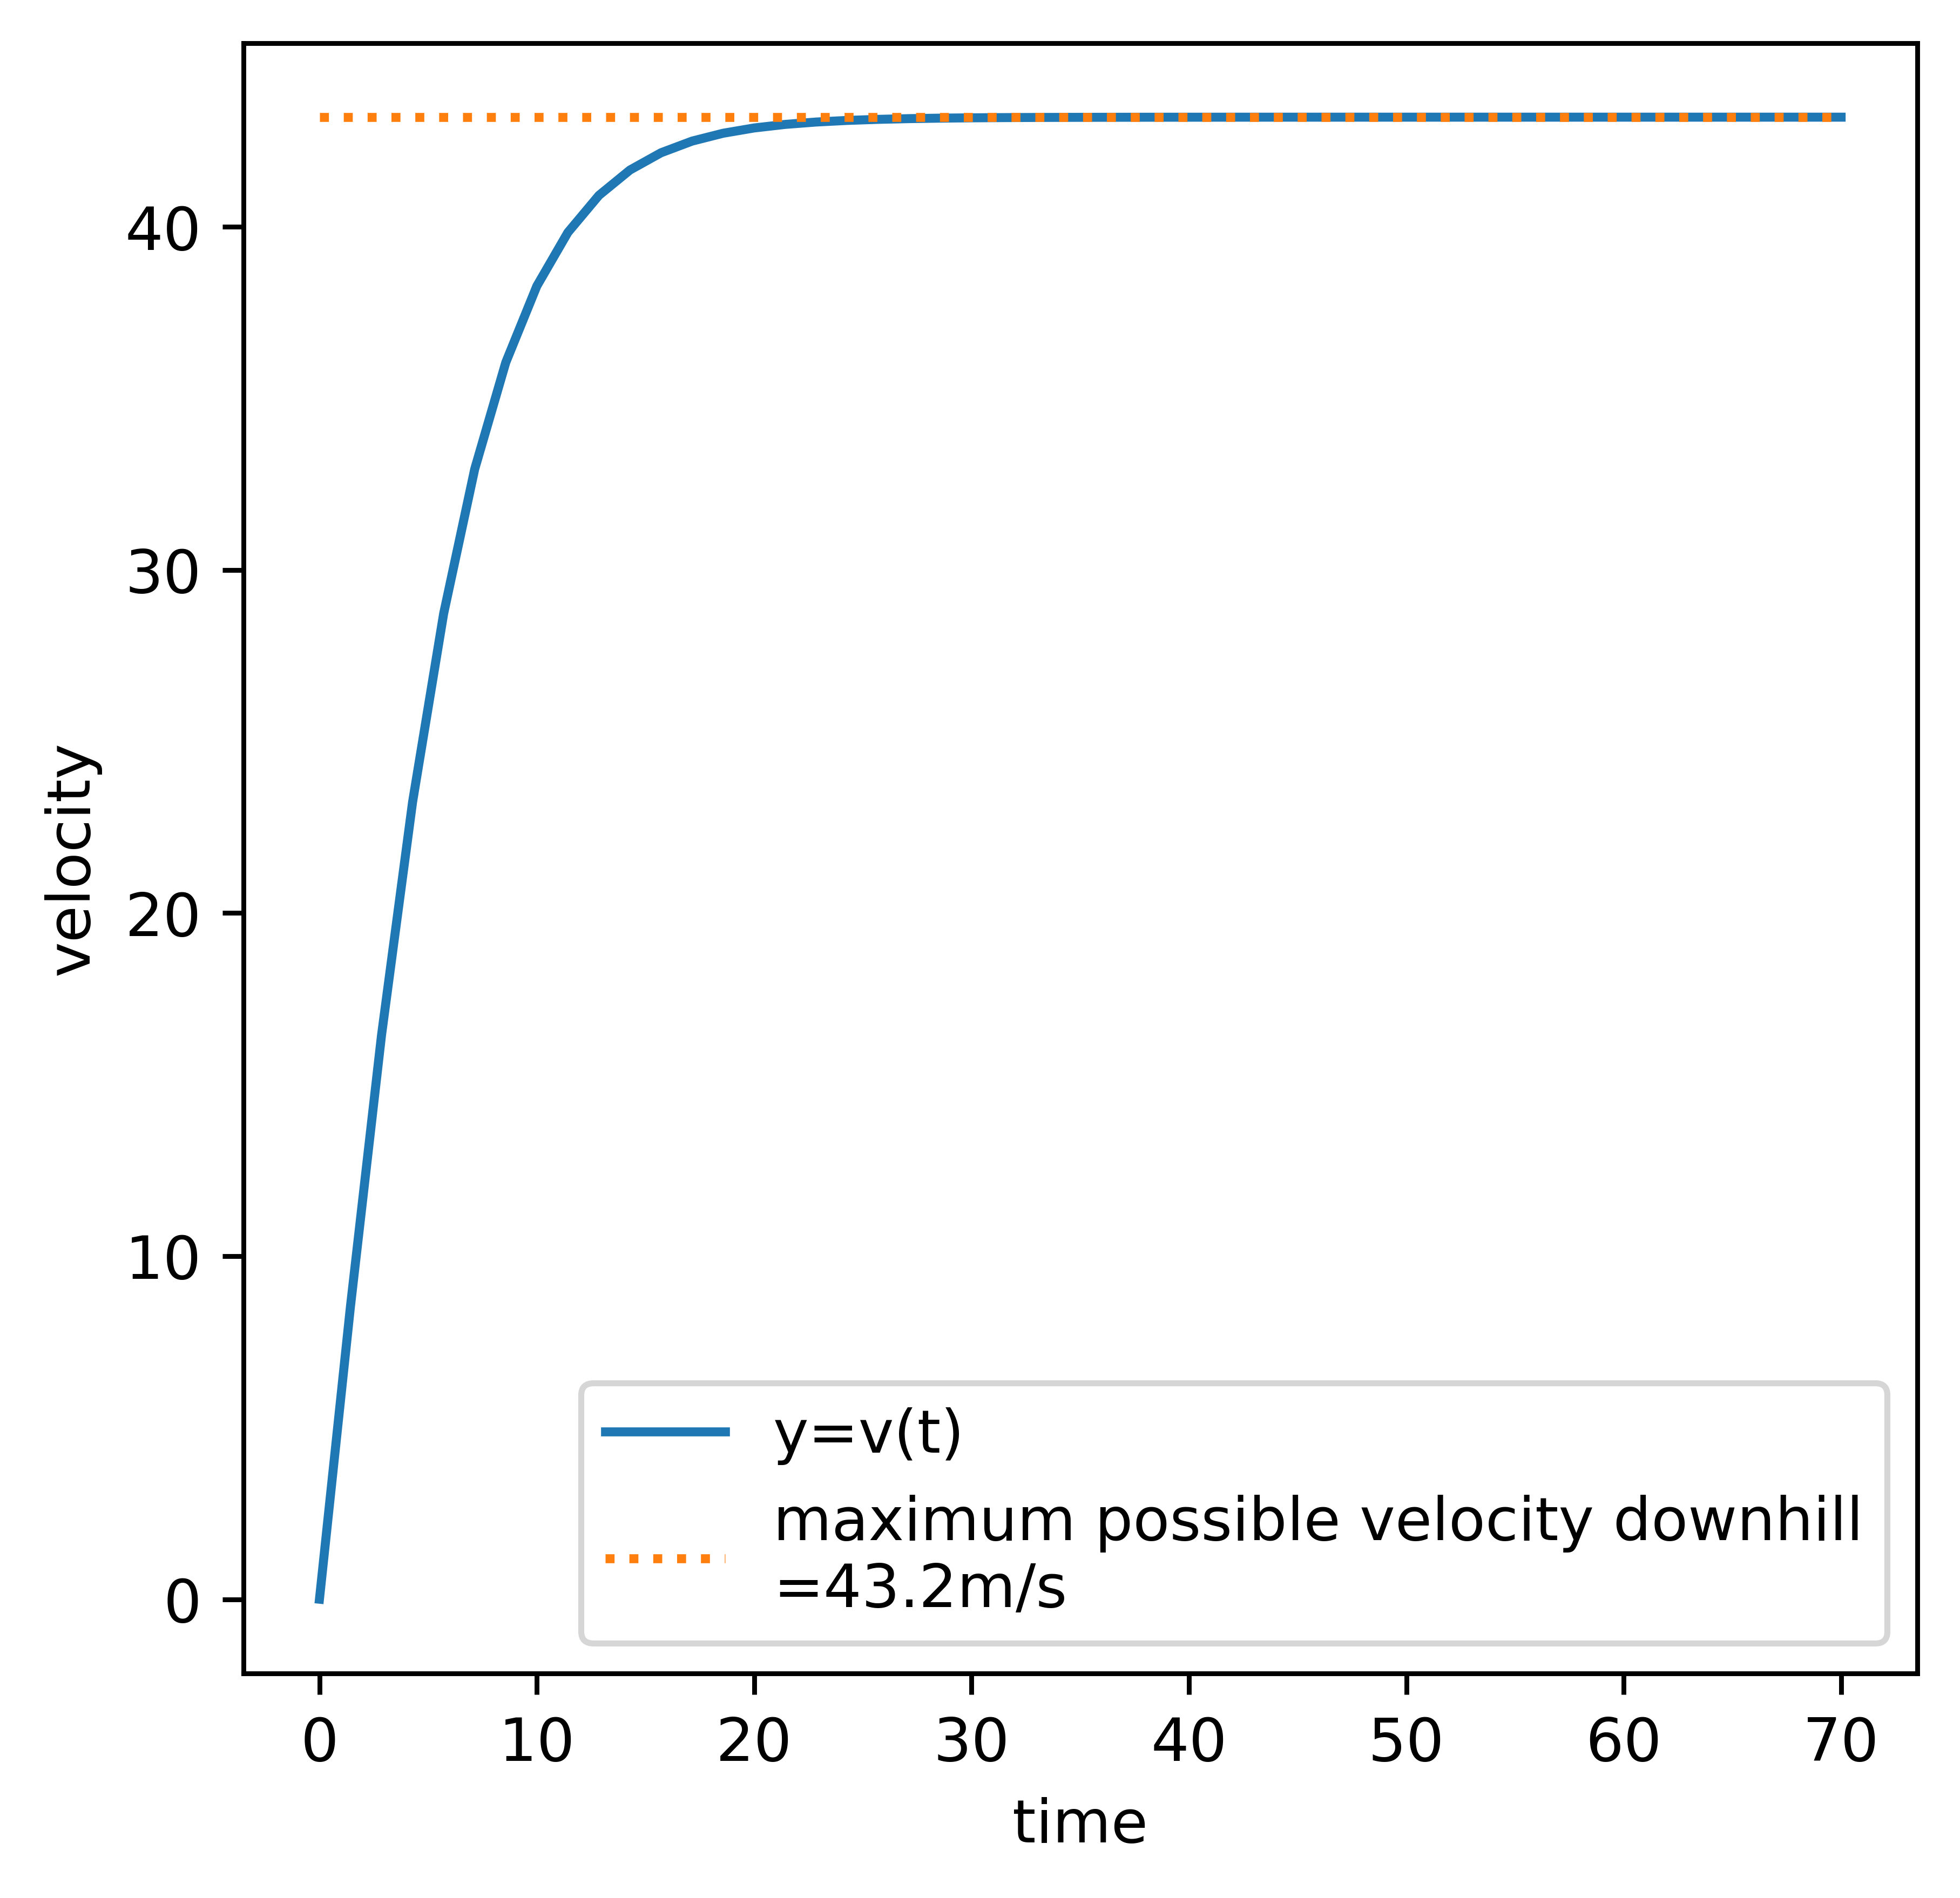
\includegraphics[height = 6cm]{9.png}

						\small \textit{Fig. 7 Velocity pattern while dashing downhill}
					\end{center}

					\begin{itemize}
						\item For the downhill part, we define \(\theta\) as the downhill slope. Therefore, we only need to change the sign before any \(\sin\left(\theta\right)\) term. After altering the formulae, we get the plot above.
						\item We divide the rest of the \textit{long} uphill slope (or plane) into three phases (speeding up; maintain a certain speed and dashing at \(E(t)=0\) with inertia).

							Suppose the three phases respectively ends at \(t_1\), \(t_2\), and \(t_{\mathrm{actual}}\). We have the following inter-restrictions on our variables:

							$$
							\begin{cases}
								E\left( t \right) =0,\:\:\forall \:t_2\le t\le t_{\mathrm{actual}}\\
								v_{\sec\mathrm{ond}\:\:\mathrm{phase}}\left( t \right) \equiv v_{\mathrm{first}\:\:\mathrm{phase}}\left( t_1 \right)\\
							\end{cases}
							$$
							\begin{enumerate}
								\item \(0\leq t\leq t_1\) (the actual value of \(t_1\) will be discussed later)
									In this phase, the whole process is just like what has been discussed in the \textit{short course} part.
									\[v_1(t)=\dfrac{\sqrt{\mathrm{A}} \tan  h \left[\dfrac{\left(m C _1+t\right)\sqrt{\mathrm{A}k}}{m}\right]}{\sqrt{ k }},\:\:0\leq t\leq t_1\]
									and with this formula, it's easy for us to get the velocity pattern before we turn into the next phase. But first let's see what'll happen during phase 3:
								\item \(t_2\leq t\leq t_{\mathrm{actual}}\) (the actual value of \(t_2\) will be discussed later)
									We use the restriction \(E_{\mathrm{third\:\:phase}}\equiv 0\), and therefore:
									\[0=E \dot(t)=\sigma-\left(f+mg\sin\theta+\dfrac{mgu}{r_{\mathrm{wheel}}}\right)\cdot v_3(t)\]
									Substitute the derivative of \(v_3(t)\) into \(m \cdot v\dot(t)=\underset{\mathrm{which\:\:equals\:\:}0}{\underbrace{\dfrac{P (t)}{v}}}-\dfrac{1}{2} k_{\mathrm{air}} v^2-mg\sin\left(\theta\right)\)
									, we solve that:

									\[v_3\left( t \right) =\sqrt{\left( v_2-\dfrac{\sigma}{k_{\mathrm{air}}} \right) \cdot e^{-2\left( t-t_2 \right) \cdot k_{\mathrm{air}}}+\dfrac{\sigma}{k_{\mathrm{air}}}}\]


								\item \(t_1\leq t\leq t_2\)
									We calculate the whole distance of the process using integral:
									\[D(v(t))=\int_0^{t_1}v_1(t)dt+v_2(t_2-t_1)+\int_{v_2}^{t_{\mathrm{actual}}}v_3(t)dt\]
									which is because \(v_2(t)\) remains a constant during the second phase.
								\end{enumerate}
							Therefore, what we need to solve is equivalent to the maximum of \(D_1+D_2+D_3\). It can also be written as:

							\[
								\begin{cases}
									\dfrac{\partial}{\partial t_1}\left( \displaystyle\sum\limits_{\mathrm{phase}}{D_i\left( t_1,t_2 \right)} \right) =0\\
									\dfrac{\partial}{\partial t_2}\left( \displaystyle\sum\limits_{\mathrm{phase}}{D_i\left( t_1,t_2 \right)} \right) =0\\
								\end{cases}\Rightarrow \left( t_1,t_2 \right)
							\]
							After getting \(t_1\) and \(t_2\), we plot the whole process into the following diagram:

							\begin{center}
								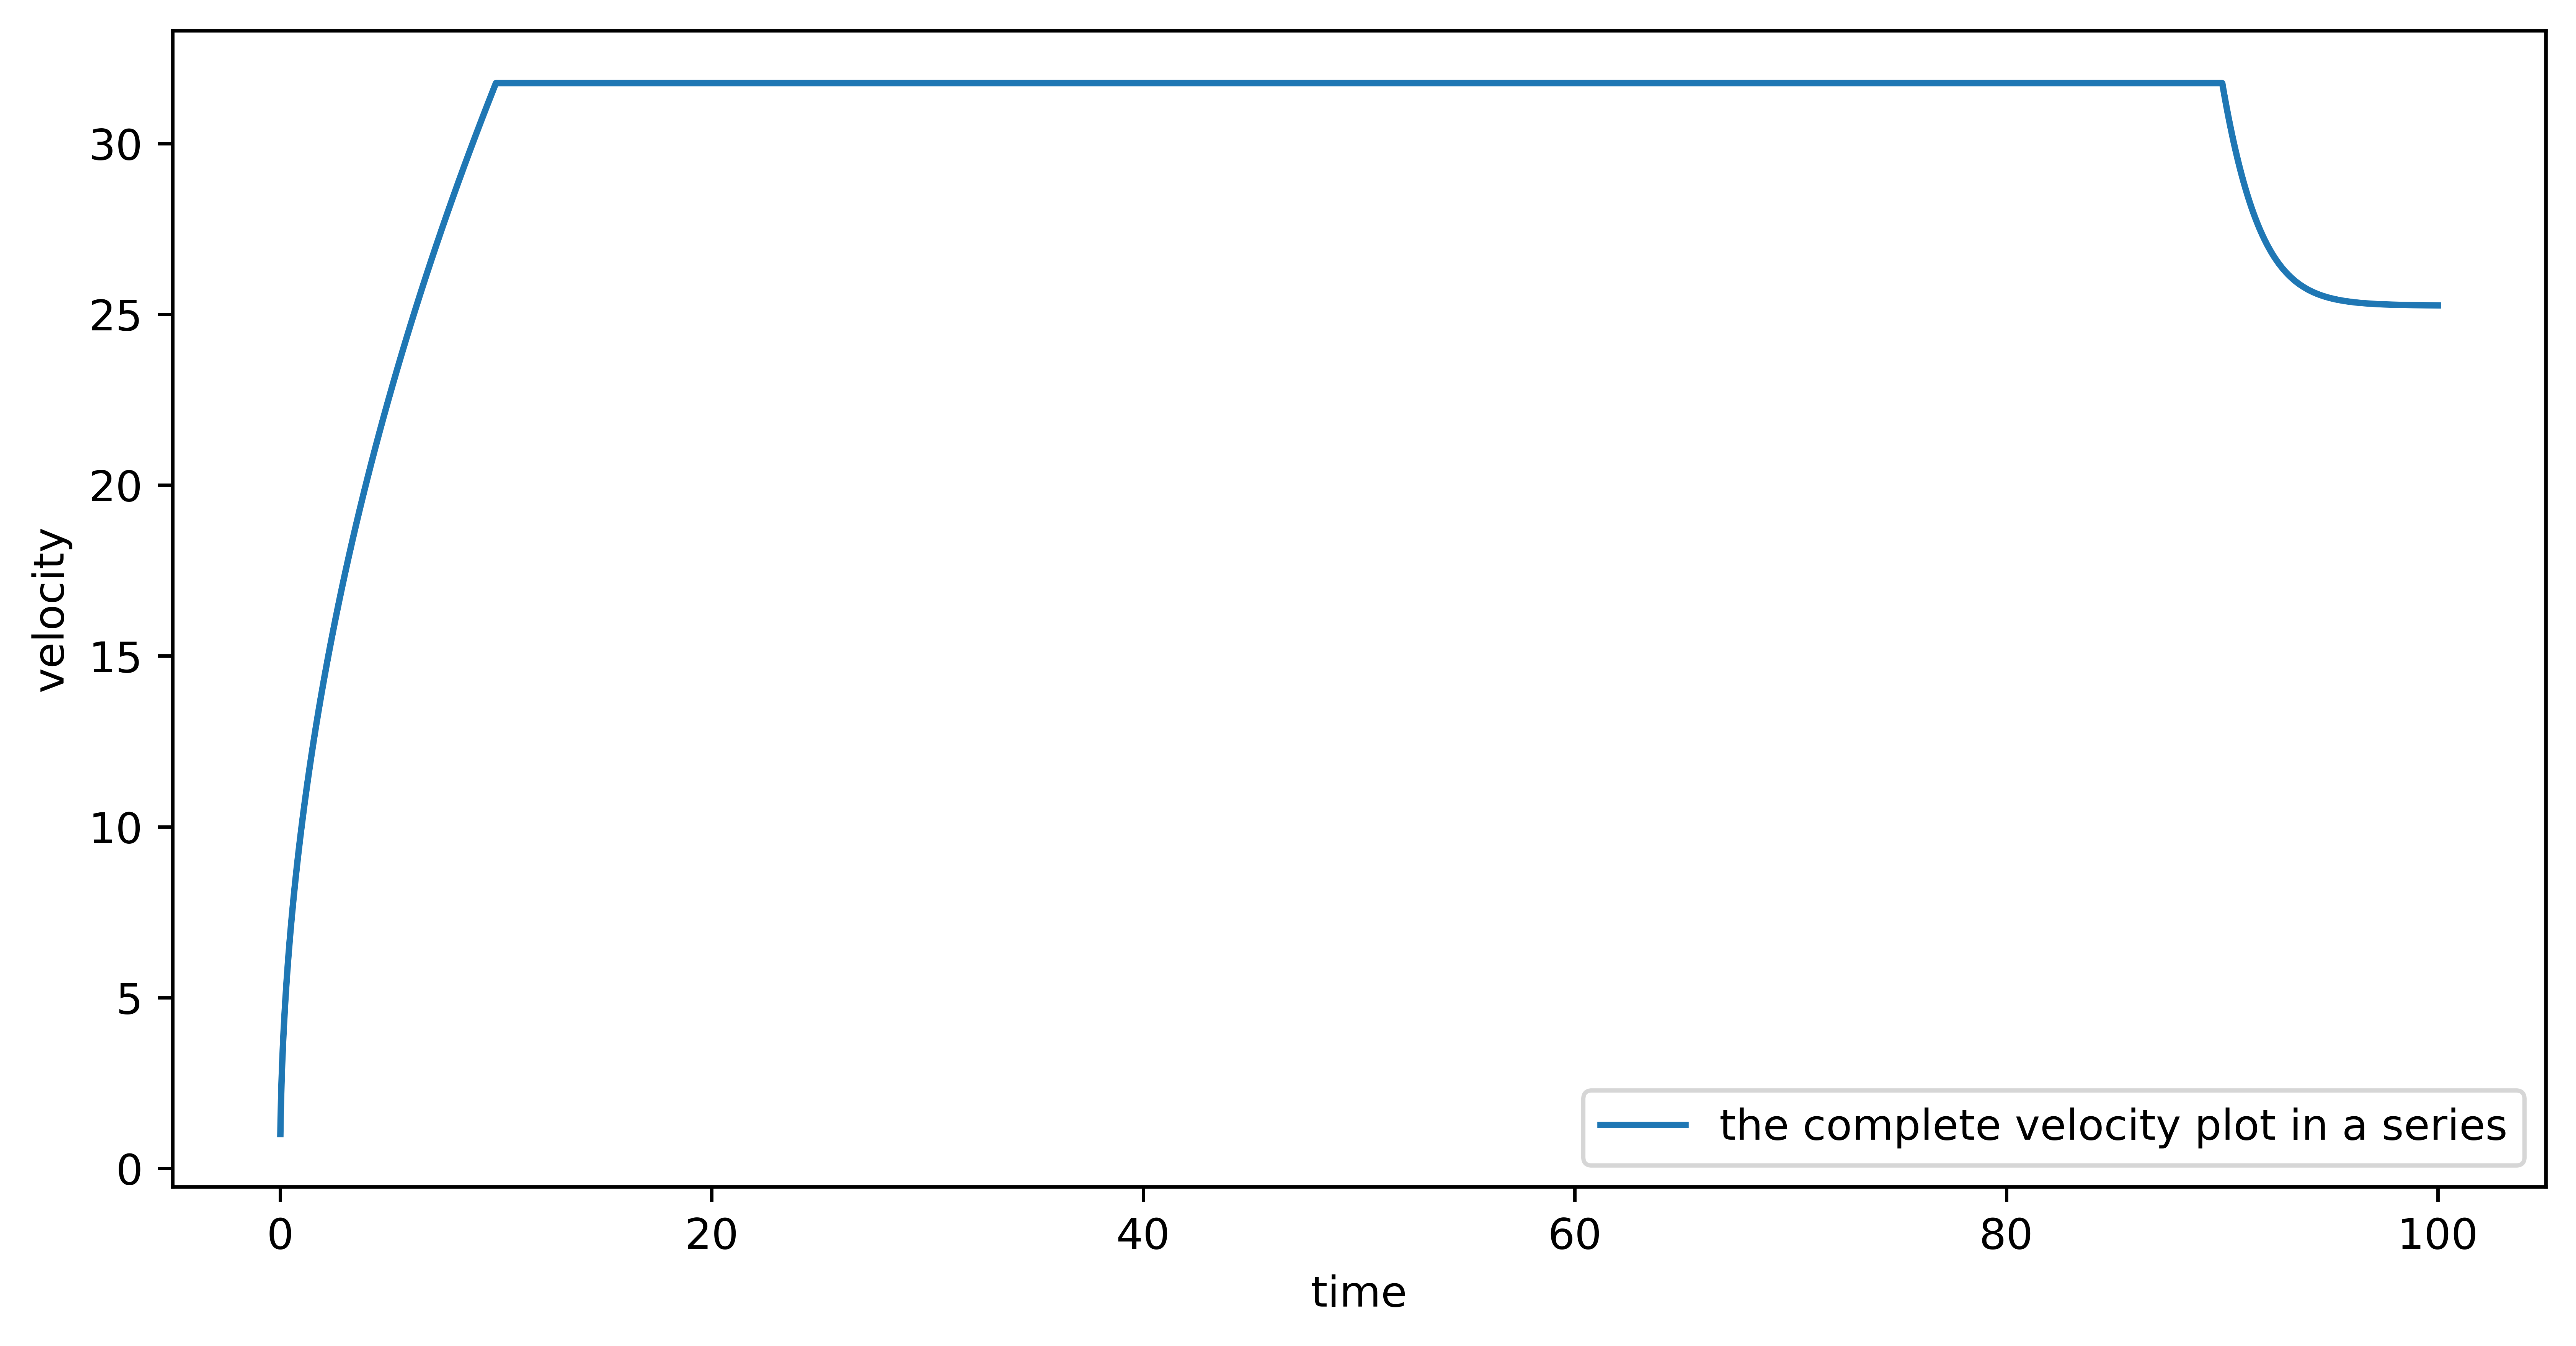
\includegraphics[height=5.5cm]{complete velocity pattern.png}

								\small\textit{Fig. Complete pattern of velocity during a series}
							\end{center}

					\end{itemize}

			\end{itemize}
		\subsubsection{splicing}
			Now that we've successfully developed a set of strategies that can be applied to a single slope or plain. To get the whole picture of \(v(t)\), we need to divide the whole course into several \defword{series} as mentioned above. Therefore, a clear definition of a \defword{turning point} is needed.

			After this, for a specic course plot, we connect all the adjacent \defword{turning points} and apply our strategies to each of the connected segments, only with these two variables changed:
			$$
			\left\{ \begin{array}{c}
				v\prime\left( 0 \right) =v_{\mathrm{end}\:\:\mathrm{of}\:\:\mathrm{last}\:\:\sec\mathrm{tion}}\\
				E\prime\left( 0 \right) =E_{\mathrm{end}\:\:\mathrm{of}\:\:\mathrm{last}\:\:\sec\mathrm{tion}}\\
			\end{array} \right.
			$$
			On a sequence of two adjacent series with the similar velocity pattern, the result is shown below:
			\begin{center}
				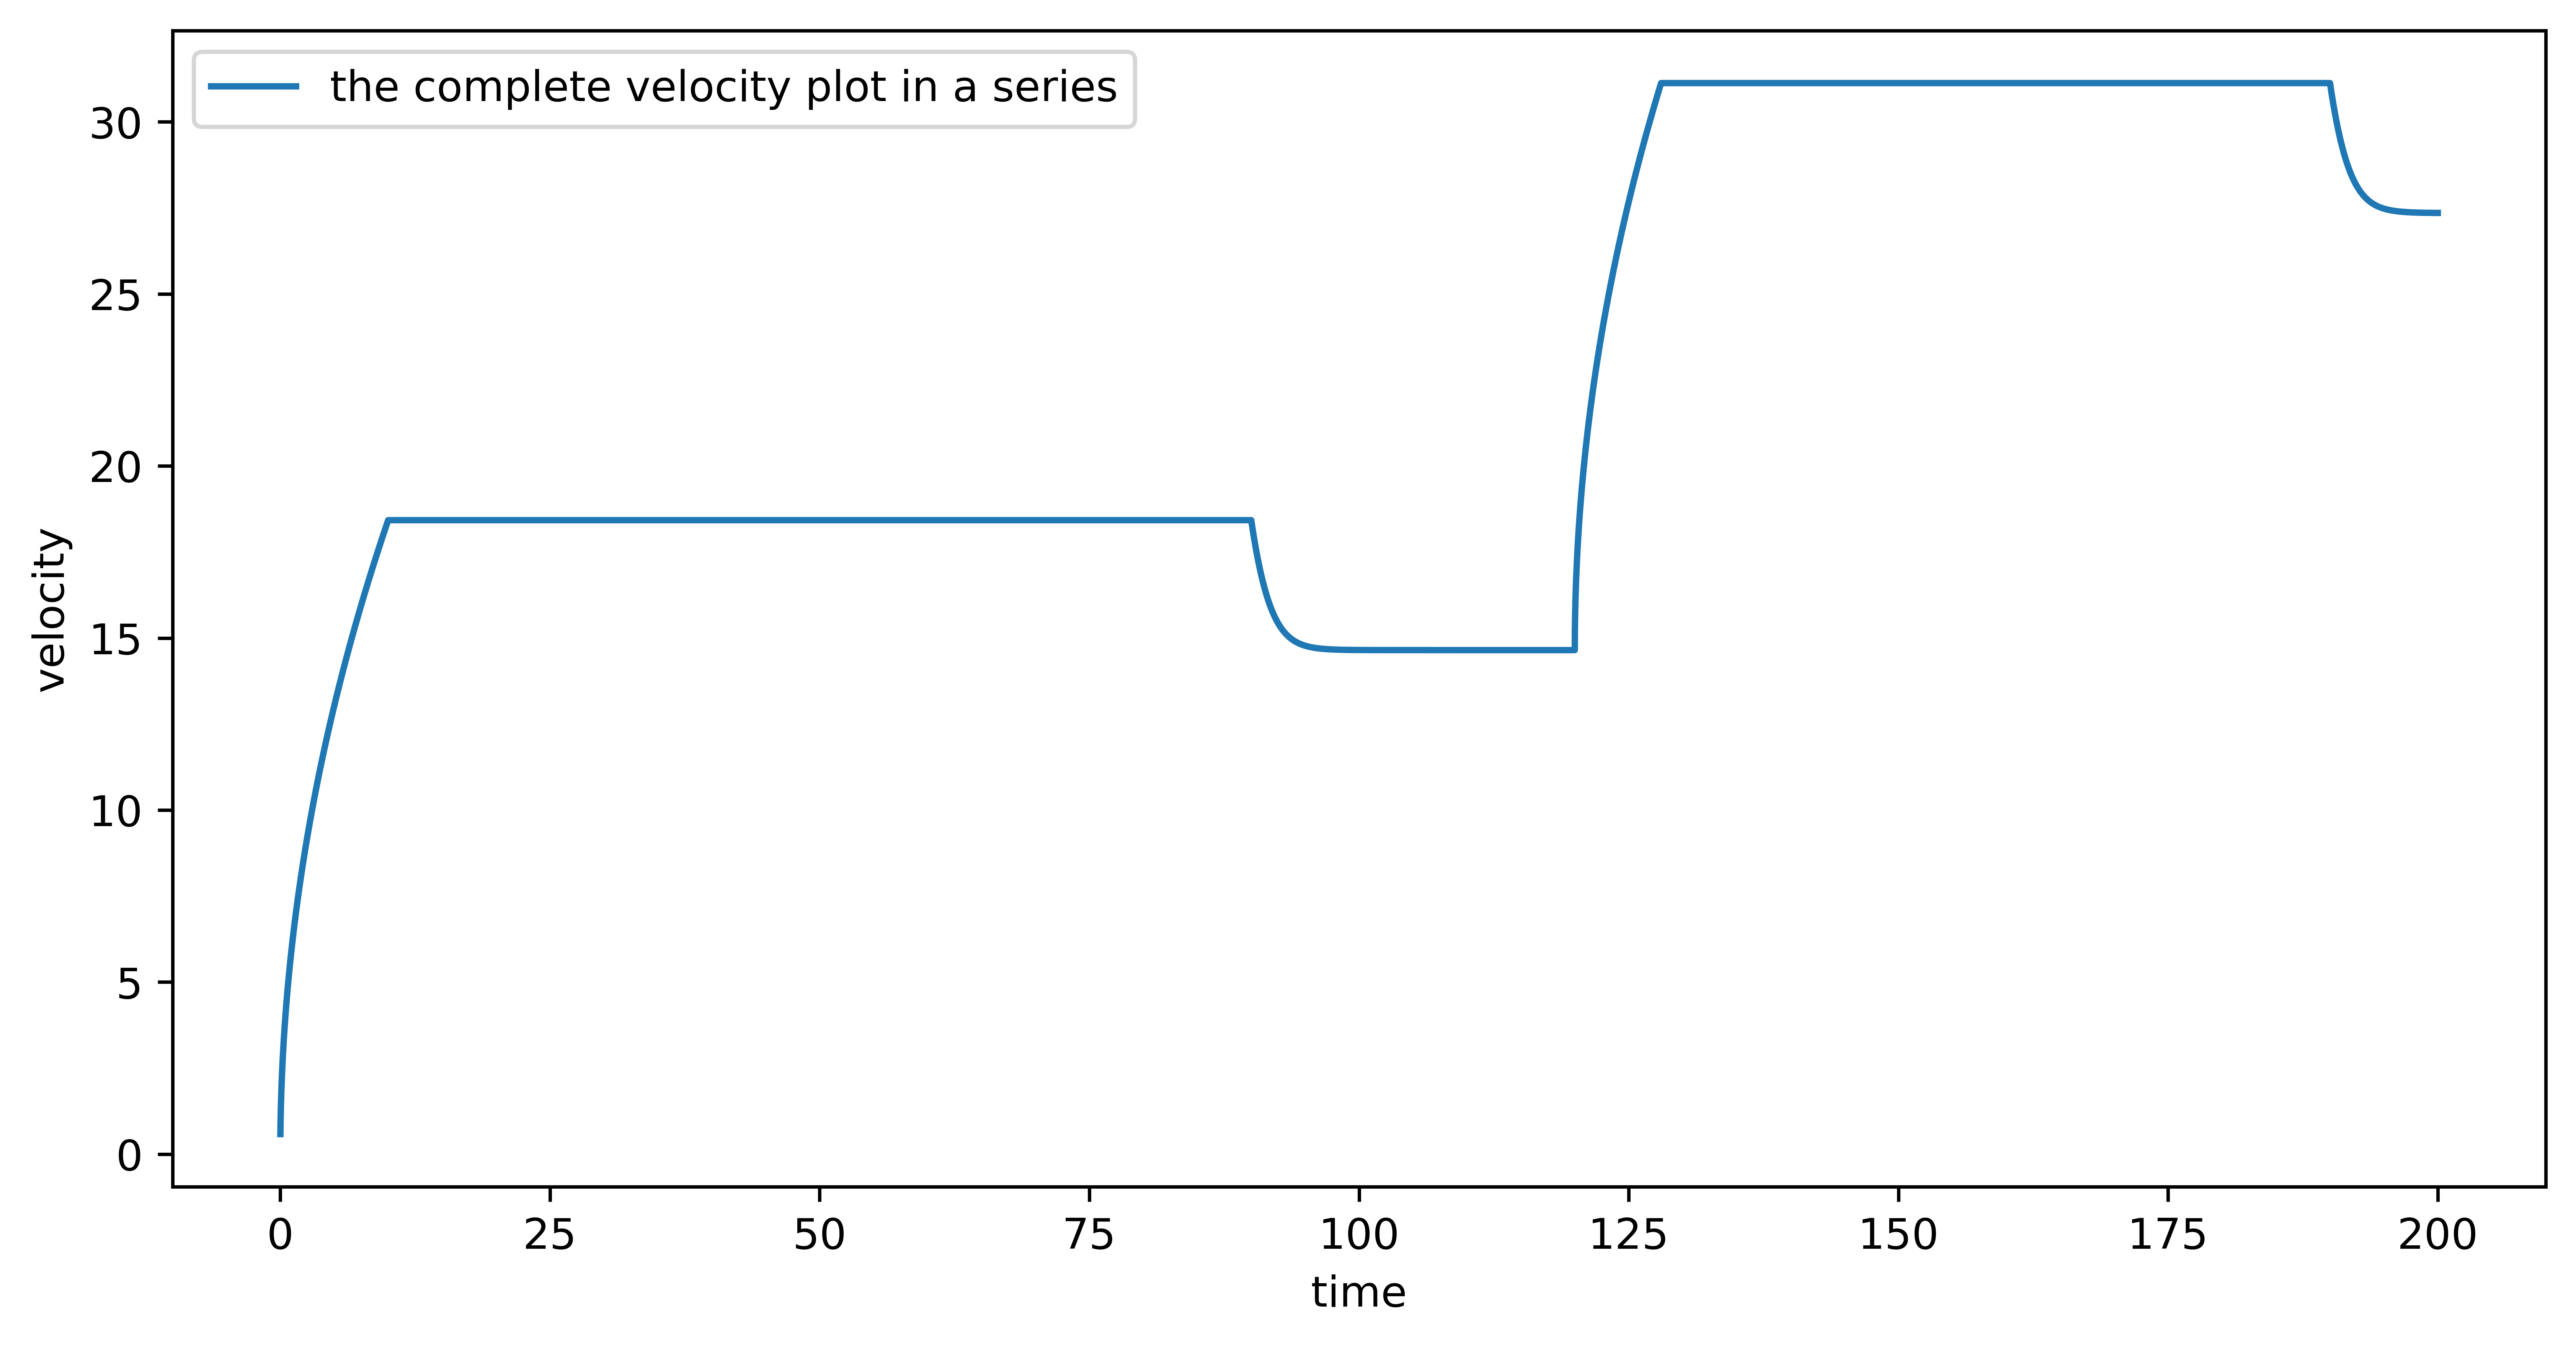
\includegraphics[height=6cm]{the complete velocity pattern in two adjacent series.png}

				\small\textit{Fig. The complete velocity pattern in two subsequent series}
			\end{center}

			However, it's also important to note that the \textit{splicing} only works well with relatively regular (especially, \textbf{linear}) changes in the slopes. Those with irregular courses will be discussed in the next model.


		\subsubsection{results on self-designed courses}
			Under the requirements in the problem, we first designed our own course. As different types of coursed are needed to respectively justify model A and B, we chose to create a more representative course that meets the \textit{almost linear pattern of slopes} condition as mentioned above. Note that with this pattern, model A actually outperforms model B on both accuracy and calculation speed.

			Below is given the \textit{bird's-eye view} of the self-designed course (but instead of the horizontal distance one might see from a vertical perspective, the label of numbers on each \defword{series} represents the actual length of that course):

			\begin{center}
				\includegraphics*[width=15cm]{8.png} \\
				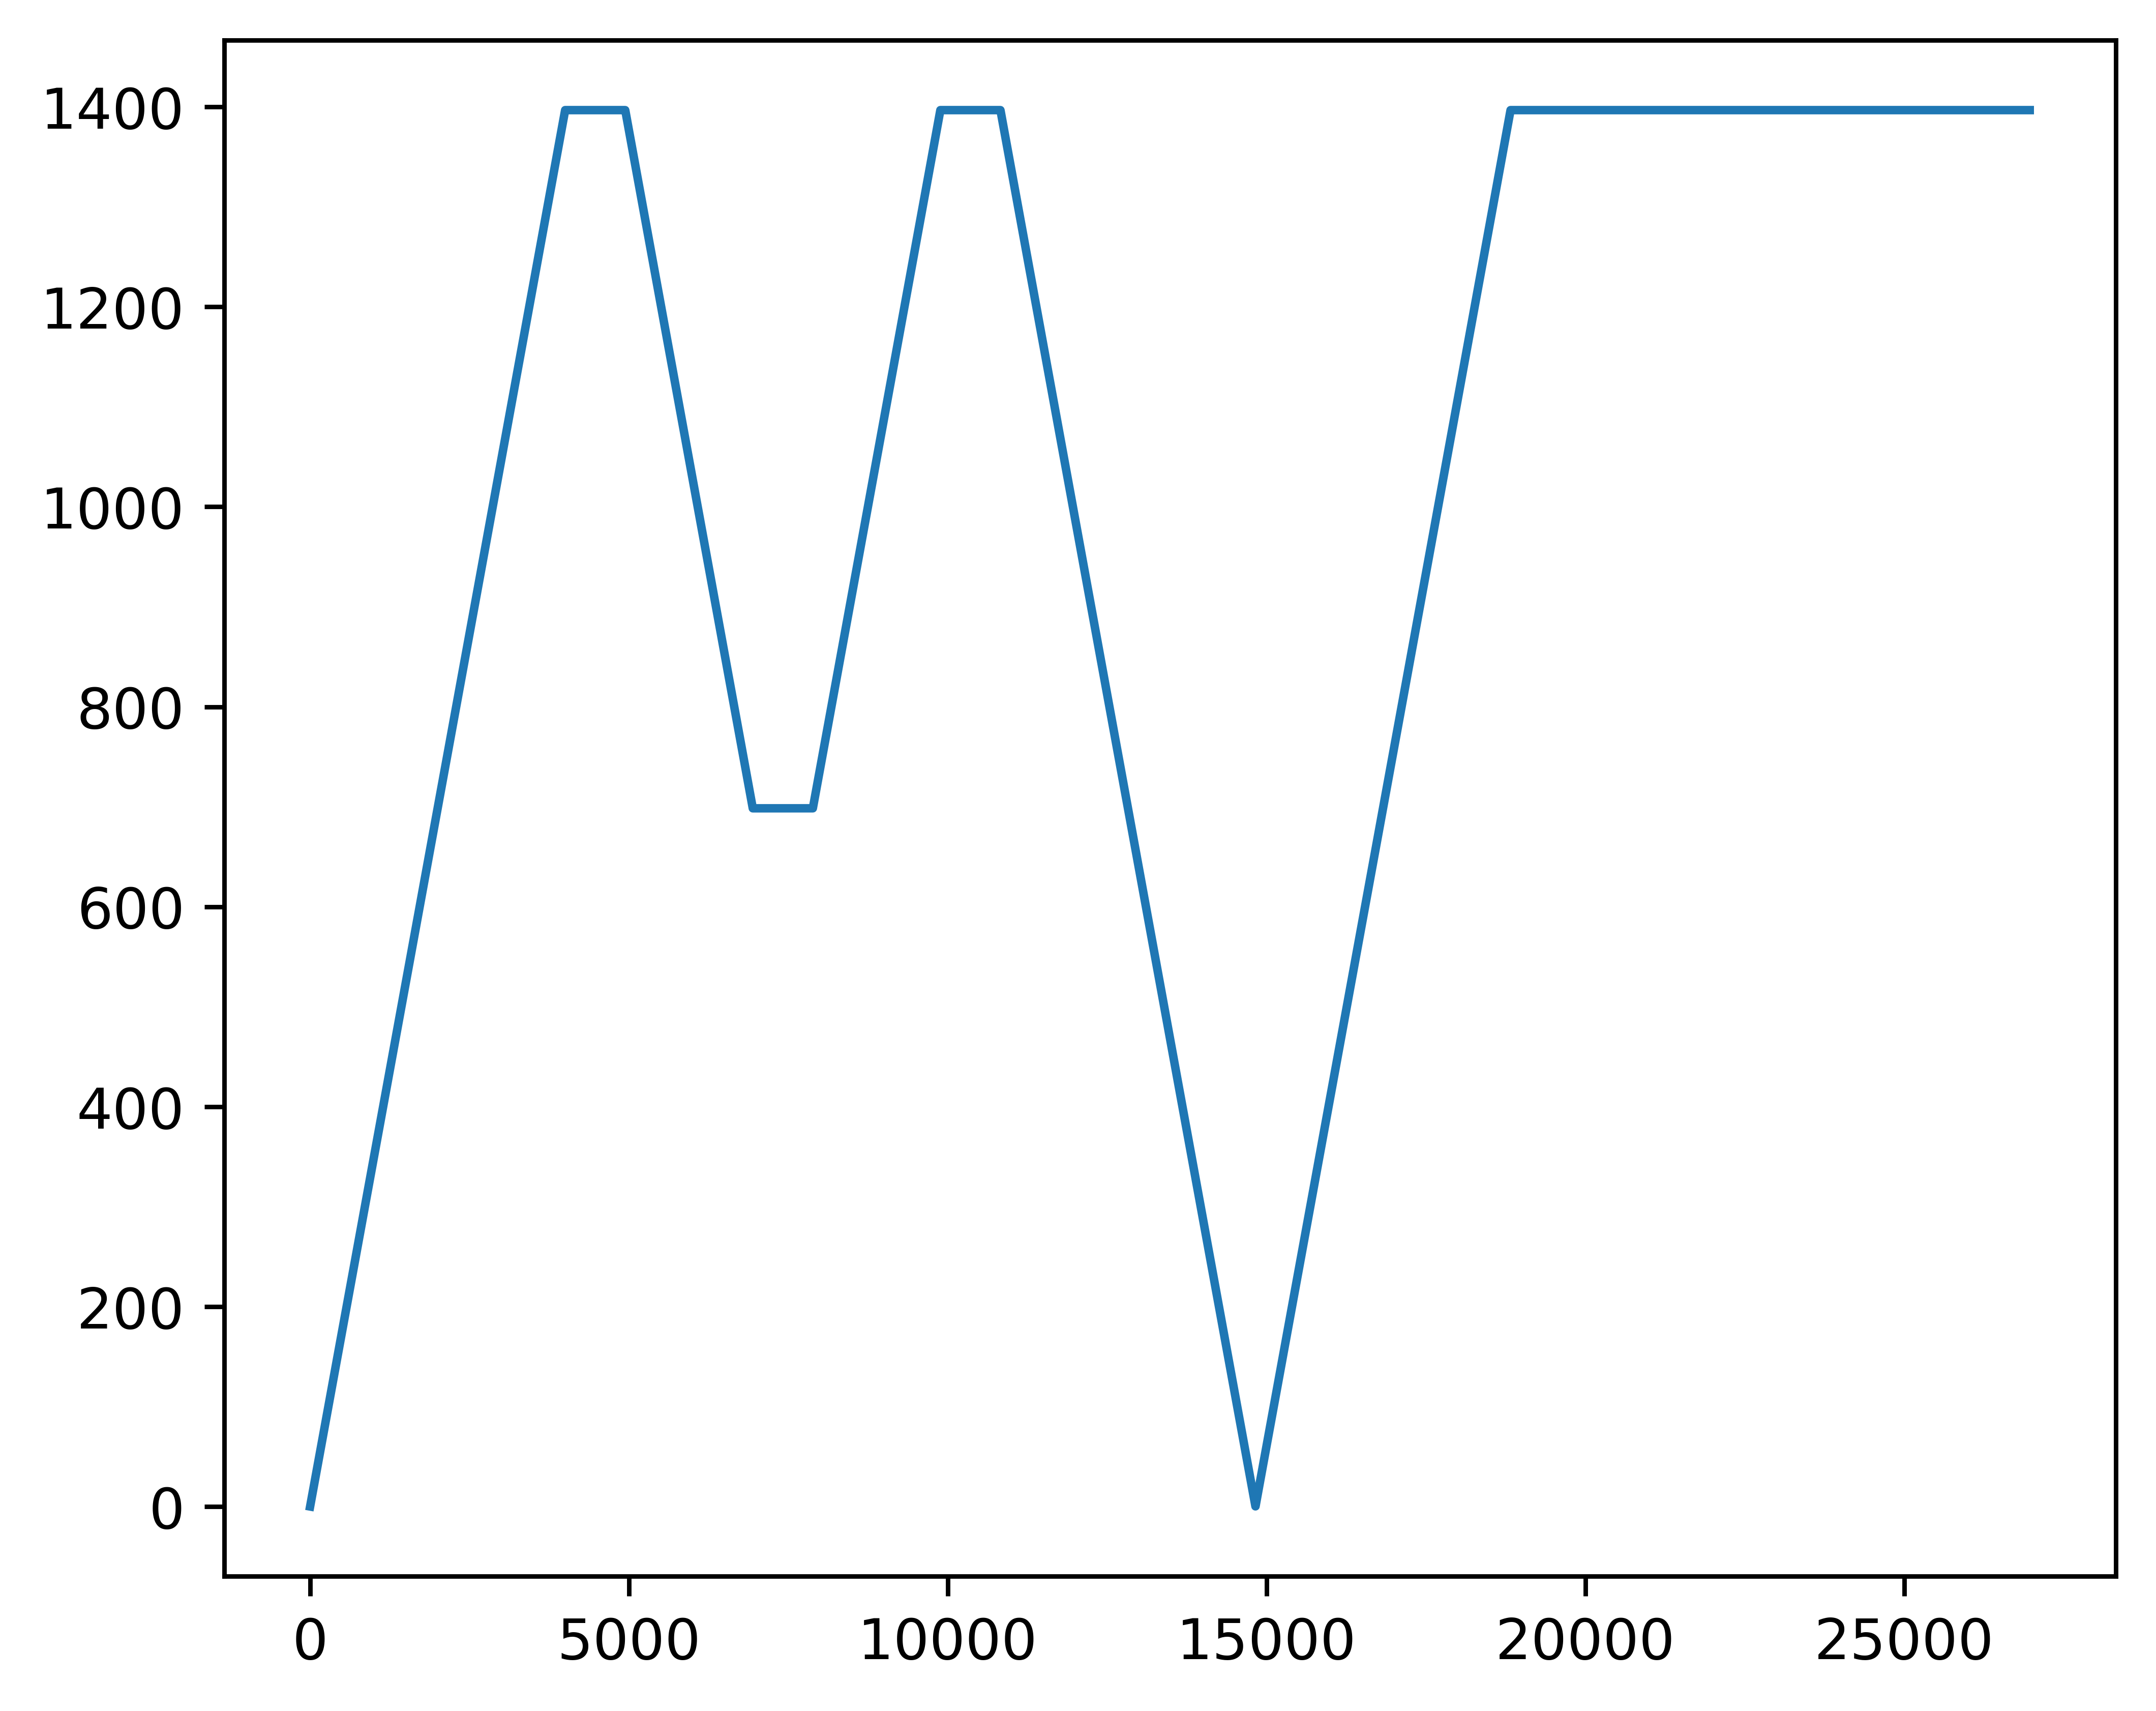
\includegraphics[width=8cm]{diycourse.png}\\

				\small\textit{Fig. DIY Course \& the elevation pattern}
			\end{center}

			\Huge ADD RESULTS\normalsize
			%\newpage
	\section{Model B}
		\subsection{Model Overview}
			In this model, we will firstly discuss how to descibe rider's basic feature and their power curve in detail. Later, we will also take special factors such as climate ino consideration. Finally, we will apply our model into several world-famous time trial courses to justify our deductions. As mentioned above, model B is applicable to all patterns of slopes, making it more universal but also more complicated than model A.
		\subsection{Assumptions}
			\begin{enumerate}
				\item	\textbf{Raining is not considered in this model.}

						Many activities have been cancelled or delayed because of rainy days in the past few years. But if the trial's humidity is under the criteria. Roads' dynamic coefficient of friction won't be affected.
				\item \textbf{The change in air density and air pressure can be neglected}

						Unlike mountain bike races, the change in altitude is small enough (\(\leq 200\mathrm{m}\)) to be neglected in the atmospherical scope.

			\end{enumerate}
		\subsection{Notation}
			\begin{tabular}{|l|l|l|}
				\hline
				$m( x )$&weight of cyclist&$\mathrm{kg}$\\
				\hline
				$ h ( x )$&height of cyclist&$\mathrm{m}$\\
				\hline
				$\mathrm{BMI}( x )$&body mass index of cyclist&/\\
				\hline
				$ E _\mathrm{total} ( x )$&total energy of cyclist&$\mathrm{J}$\\
				\hline
				$\mathrm{S}_\mathrm{body}( x )$&body measure&$\mathrm{m}^2$\\
				\hline
				$\tau_{\mathrm{min}}$&the least time spent to complete the game&$\mathrm{s}$\\
				\hline
				$F_\mathrm{wind}$&wind force&$\mathrm{N}$\\
				\hline
				$\tau$&temperature of the trial&$^\circ\mathrm{C}$\\
				\hline
				$\mathrm{K}_ b $&the Boltzmann constant&/\\
				\hline
				\(L\) & the learning rate of an individual cyclist, or his/her adaptability to different terrains & /\\
				\hline
				\(\epsilon\) & attenuation factor & /\\
				\hline
			\end{tabular}
		\subsection{Individual Factors}
			In this part, we will mainly discuss the cyclist's total power based on his/her phisycal condition and the type of cyclist he/she is. The relative attributes of an individual cyclist are listed below:

			\[\boxed{\mathrm{rider\:\:classification\:\:system}} \rightarrow \begin{cases}
				\mathrm{Gender}\left( x \right)\\
				\mathrm{Weight}\left( x \right)=m(x)\\
				\mathrm{Height}\left( x \right)=h(x)\\
				\mathrm{Age}\left( x \right)\\
				\mathrm{Type}\left( x \right) \rightarrow \begin{cases}
				L=\mathrm{Learning}\:\:\mathrm{rate}\\
				\epsilon\:\:(\mathrm{how\:\:capable\:\:he/she\:\:is\:\:at\:\:using\:\:strength})\\
			\end{cases}\\
			\end{cases}\]

			First, we need to have a basic understanding of the cyclist's physical condition. Take Tour de France as an example\cite{france}. Among the champions of this race in the past five years, their average height is 1.808$\mathrm{m}$ and their average weight is 68.58$\mathrm{kg}$. Olympic cyclists have an average height of 1.80$\mathrm{m}$ and an average of around 68$\mathrm{kg}$\cite{weight}.

			Next, we quantify the attributes of a cyclist with two indicator variables: \(L\) represents the cyclist's adaptability to new terrains, or the \textbf{learning rate}, which will later be introduced in the algorithms. The higher \(L\) is, the more quickly the rider will change his/her strategy during the course. Another indicator \(\epsilon\), which has already been mentioned before, measures the rider's capability of converting force into dynamics.

			To achieve this, we used the neural networks algorithm to get these two indicators by fitting them into previous records. Relative calculations have already done in the physical analysis part in model A. The process is shown below:

			\begin{center}
				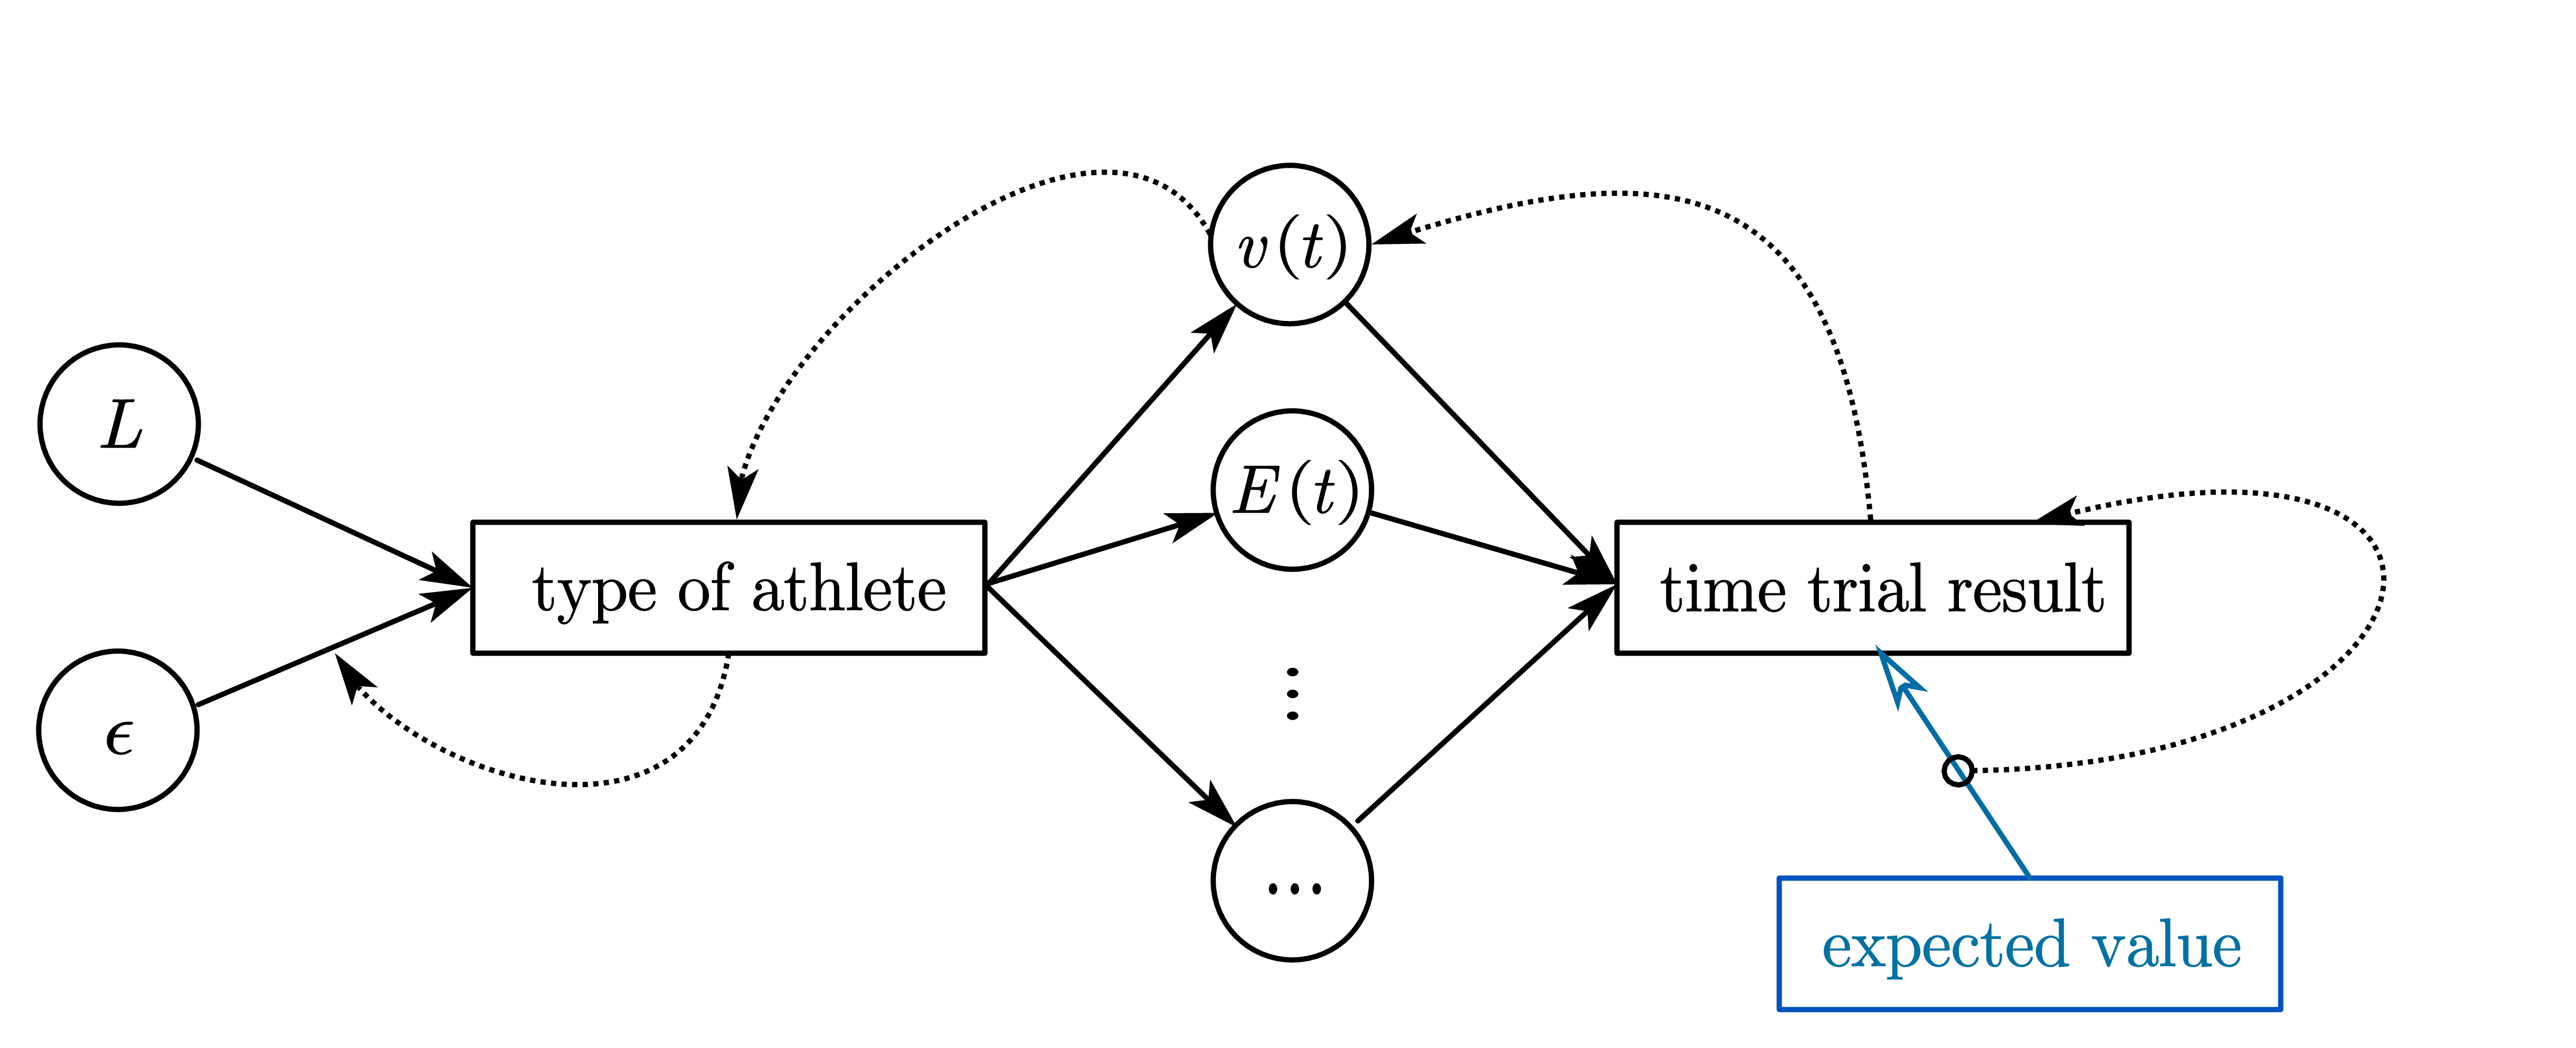
\includegraphics[height = 6cm]{neural networks.png}

				\small\textit{Fig. The working process of the neural network}
			\end{center}

			Then we randomly pick the parameters and put it into practice using the formulae:

			\begin{center}
				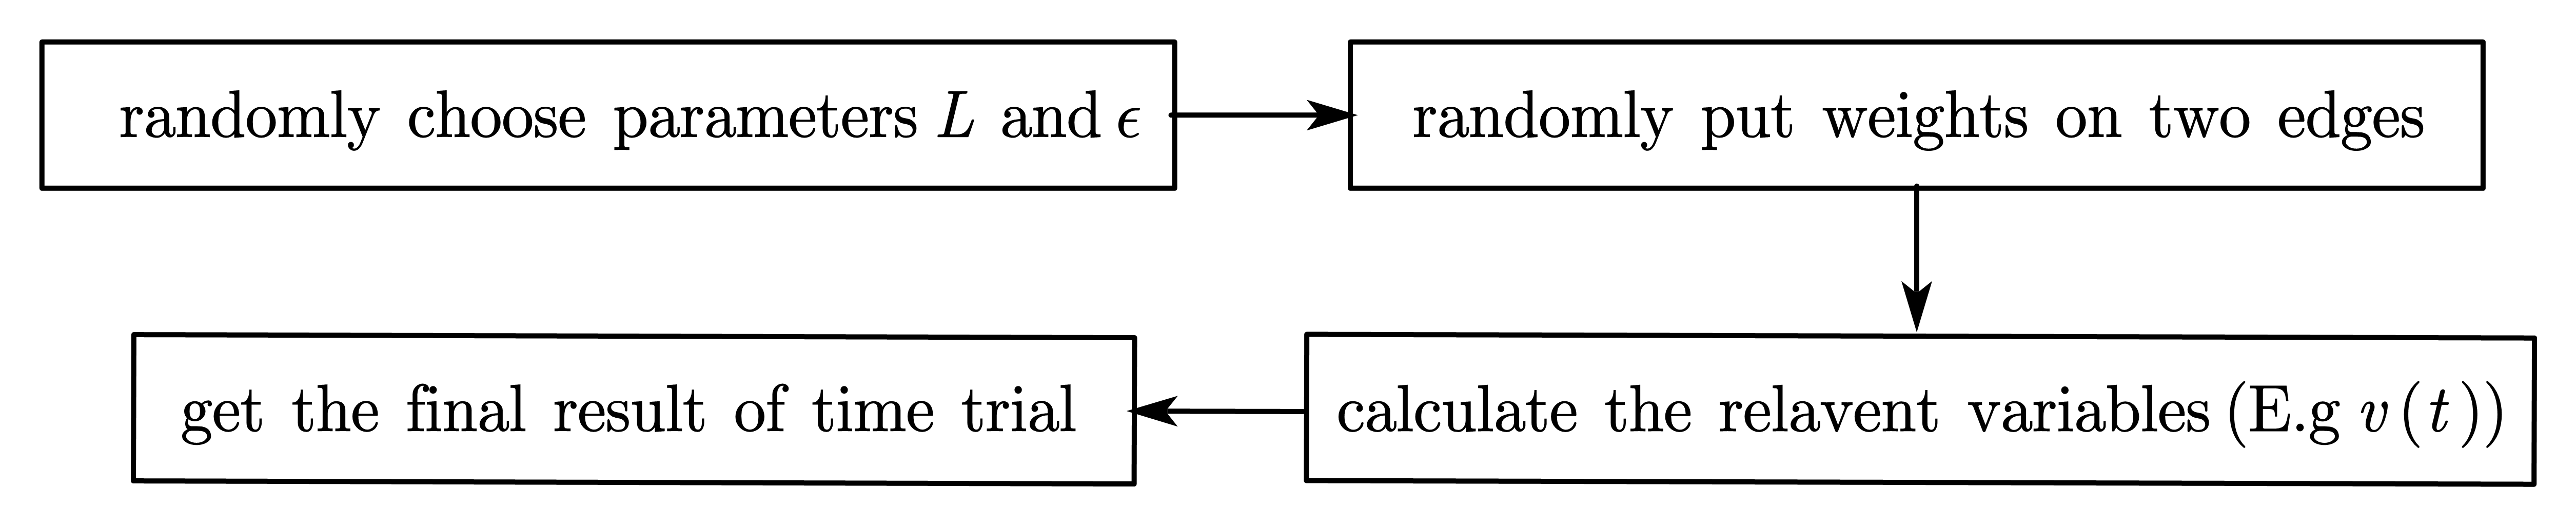
\includegraphics[width=12cm]{deciding the parameters.png}

				\small\textit{Fig. Deciding the parameters}
			\end{center}

			We compare the standard difference \(\left( r_{\exp}-r_{\mathrm{act}} \right) ^2\) between the expected value and the actual calculated one, and make renders to the parameters. In the end, we got the results when the parameters became relatively stable, as shown below:

			\begin{center}
				\begin{tabular}{|l||c|c|c|c|c|}
					\hline
					&\textbf{time trial specialist} & \textbf{climber} & \textbf{rouleur} & \textbf{sprinter} & \textbf{puncheur} \\
					\hline
					\hline
					\(L\) & 0.95 & 0.74 & 0.90 & 0.65 & 0.82 \\
					\hline
					\(\epsilon\) & 0.85 & 0.91 & 0.90 & 0.70 & 1.00 \\
					\hline
				\end{tabular}
			\end{center}

			In our model, we use a series of variables with (\(x\)) to describe the cyclist's features. These include $m( x )$, $ h ( x )$, etc. According to the BMI criteria, we can get the formula:
			$$\mathrm{BMI}( x )=\dfrac{m( x )}{ h ^2( x )}$$
			Also, since where our body is exposed to air can be seen as a rectangle, we can approximately get that:
			\[S_{\mathrm{body}} \propto \mathrm{BMI}(x)\cdot h(x)\]
			\[\Rightarrow S_{\mathrm{body}}=k\cdot \dfrac{m(x)}{h(x)}\]
			The total energy can also be given by a weighted sum of the parameters listed:
			\[E_{\mathrm{total}}=-k_1\cdot\mathrm{Gender}(x)+k_2[m(x)-w_0]^2+k_3\cdot A\cdot [\mathrm{Age}(x)]+k_4\]
			where
			\[A(x)=
				\begin{cases}
					k_5\left\{\sin\left[\dfrac{(x-15.5)\pi}{31 }\right]+1\right\}~~~,~x\leq 31 \\
					-k_6 (x-31)^2+2k_5~~~~~~~~~~~~~~,x>31
				\end{cases}
			\]
			and according to \cite{114514}, \(\max\{E_{\mathrm{total}}\}\approx 2403.5 \mathrm{J}\ddef E_{0}\). By searching the internet \cite{energy curve}, we can find that a pesron reaches his/her maximum energy at the age of 31.
			\[
				\Rightarrow
				\begin{cases}
					\lim\limits_{x\rightarrow 31^+} A\left( x \right) =\lim\limits_{x\rightarrow 31^-} A\left( x \right)=E_0 \\
					A(60)=\dfrac 12 E_0
				\end{cases}
			\]
			Therefore, \(k_5 = \dfrac{E_0}{2}\) and \(k_6=\dfrac{k_5}{841}\). The plot is shown below:
			\begin{center}
				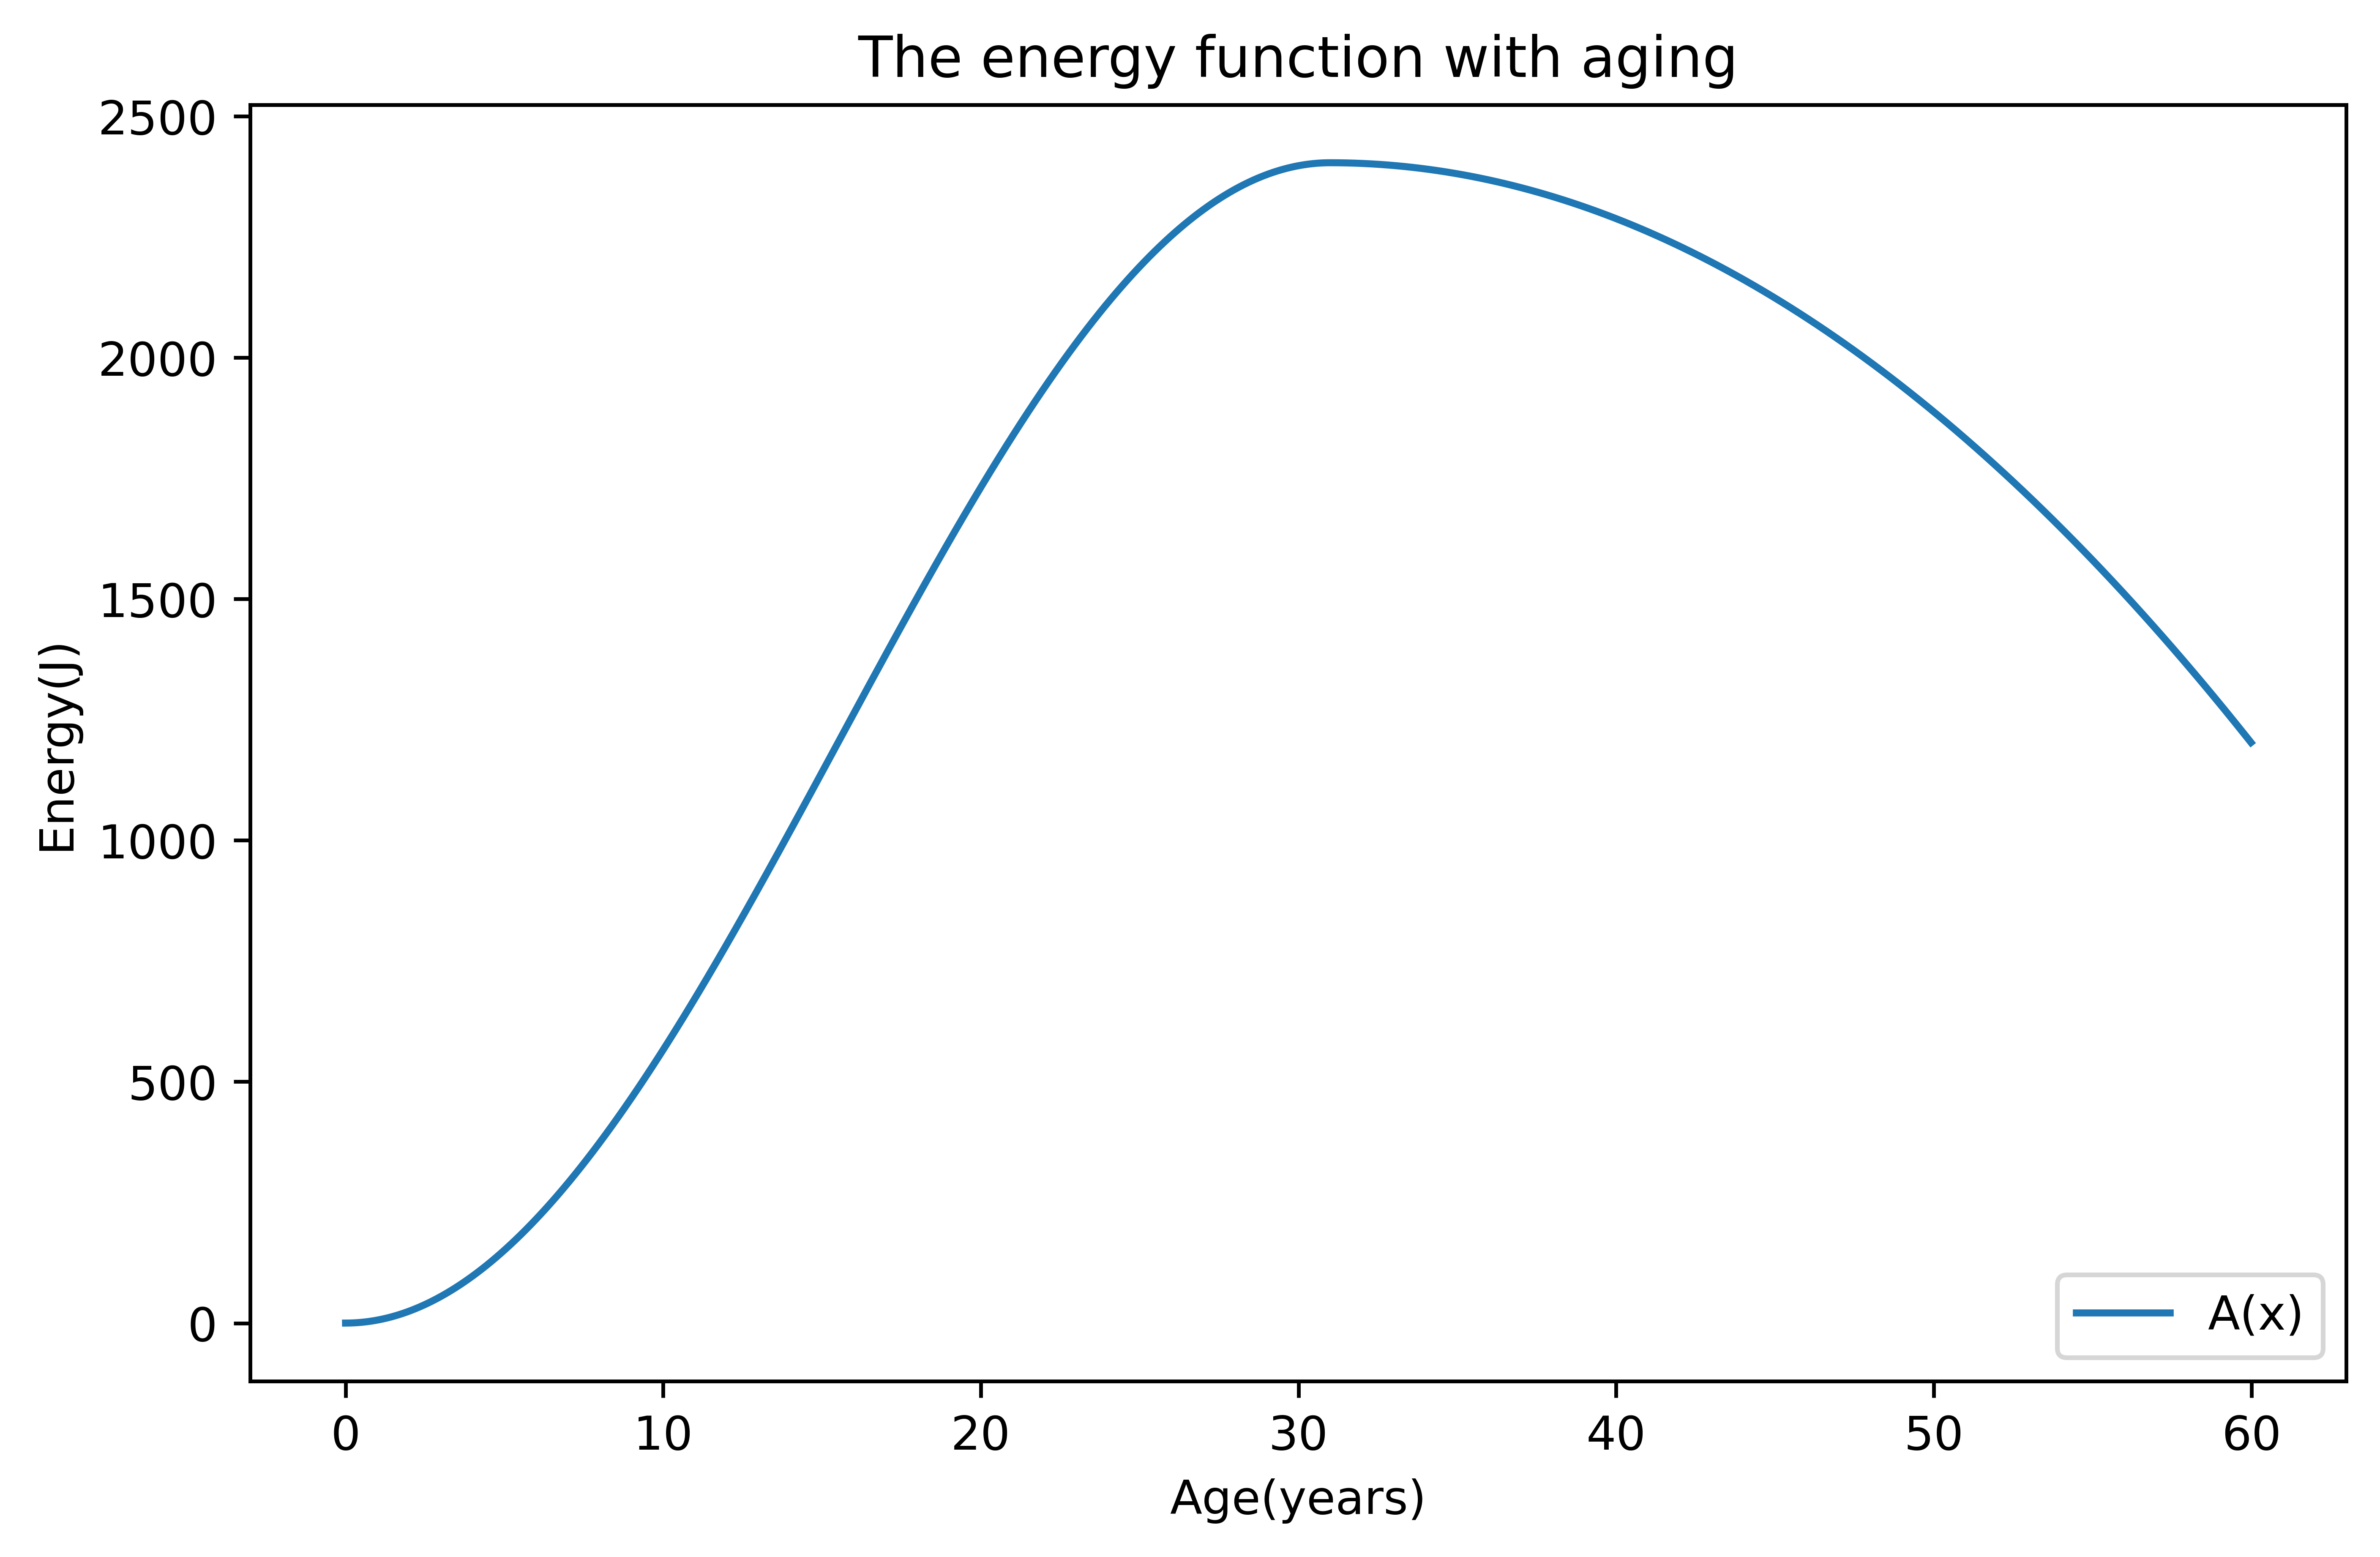
\includegraphics[height = 6cm]{energy function with aging.png}

				\small\textit{Fig. Energy function with aging}
			\end{center}

			% \begin{allanenvhypothesis}
			% 	A person at the age of 60 has half of the dispensible energy as \(E_0\).
			% \end{allanenvhypothesis}


		\subsection{Weather Conditions}
			Weather condition also plays a vital part in the cyclists's strategy. In this part, we will mianly discuss two kinds of weather condition: temperature and wind force.
		\subsubsection{Temperature}
			Temperature mainly has an impact on human's speed of metabolism. 20$^\circ \mathrm{C}$ to 30$^\circ\mathrm{C}$ is the the zone where human can complete phisical actions in the most comfortable way. If the environment's temperature is over or below whis number, speed of metabolsim will decline. The greater the difference is ,the more quickly the speed decline. Therefore we can get the following formula:
			$$\sigma\propto e^{-\dfrac{ E _\mathrm{total}}{\mathrm{K}_ b \tau}}$$
			($\mathrm{K}_ b $ here refers to the Boltz constant which equals $1.38\times10^{-16}$ per degree calcius)
		\subsubsection{Wind Force}
			Secondly, we need to discuss the wind force. Since there is wind disturbing the cyclists, w1.e can assume that air resistance no longer exists. This picture below shows the situation where a rider is facing the wind. So we can get the following formula:
			$$F_\mathrm{wind}=\rho_\mathrm{air}\cdot S_\mathrm{body}v^2$$

			Now we can analyze the cyclist's overal stress distribution, which is:

			\[F_\mathrm{total}=-\dfrac{1}{2}C_ D \rho S_\mathrm{body} v^2+C_ D \rho S_\mathrm{body}v_{wind}v-(mg\sin\theta+\dfrac{1}{2}C_ D \rho S_\mathrm{body}v_{wind}^2+\dfrac{mg\mu}{r})\]



		\subsection{Recalculating the model using real-time data}

			To make our model applicable to all courses, we notice the fact that for a set course, its slope can be calculated with the following formula:

			\[ \tan (\theta\left(t\right)) =\dot{D_{\mathrm{course}}\left( t \right) } \]

			And it made the subsequent changes to \( \sin\theta \) and \(\cos \theta\) as well. Notice that there is also an equation which connects that equation with other variables:

			\[ D_{\mathrm{course}}\left( t \right) =\int_0^t{v\left( t \right)  D t} \]

			On the other hand, on the psychological side of participants,

			Before we actually solve the differential equation above, it's also critical to observe that the consideration of \textit{psychological} factors mean that reactional delays are not proportional to time, making it difficult to actually solve the differential equation set. Therefore, we adopt the \textit{Q-Learning} algorithm do make the process dynamic, as shown below:

			\begin{center}
				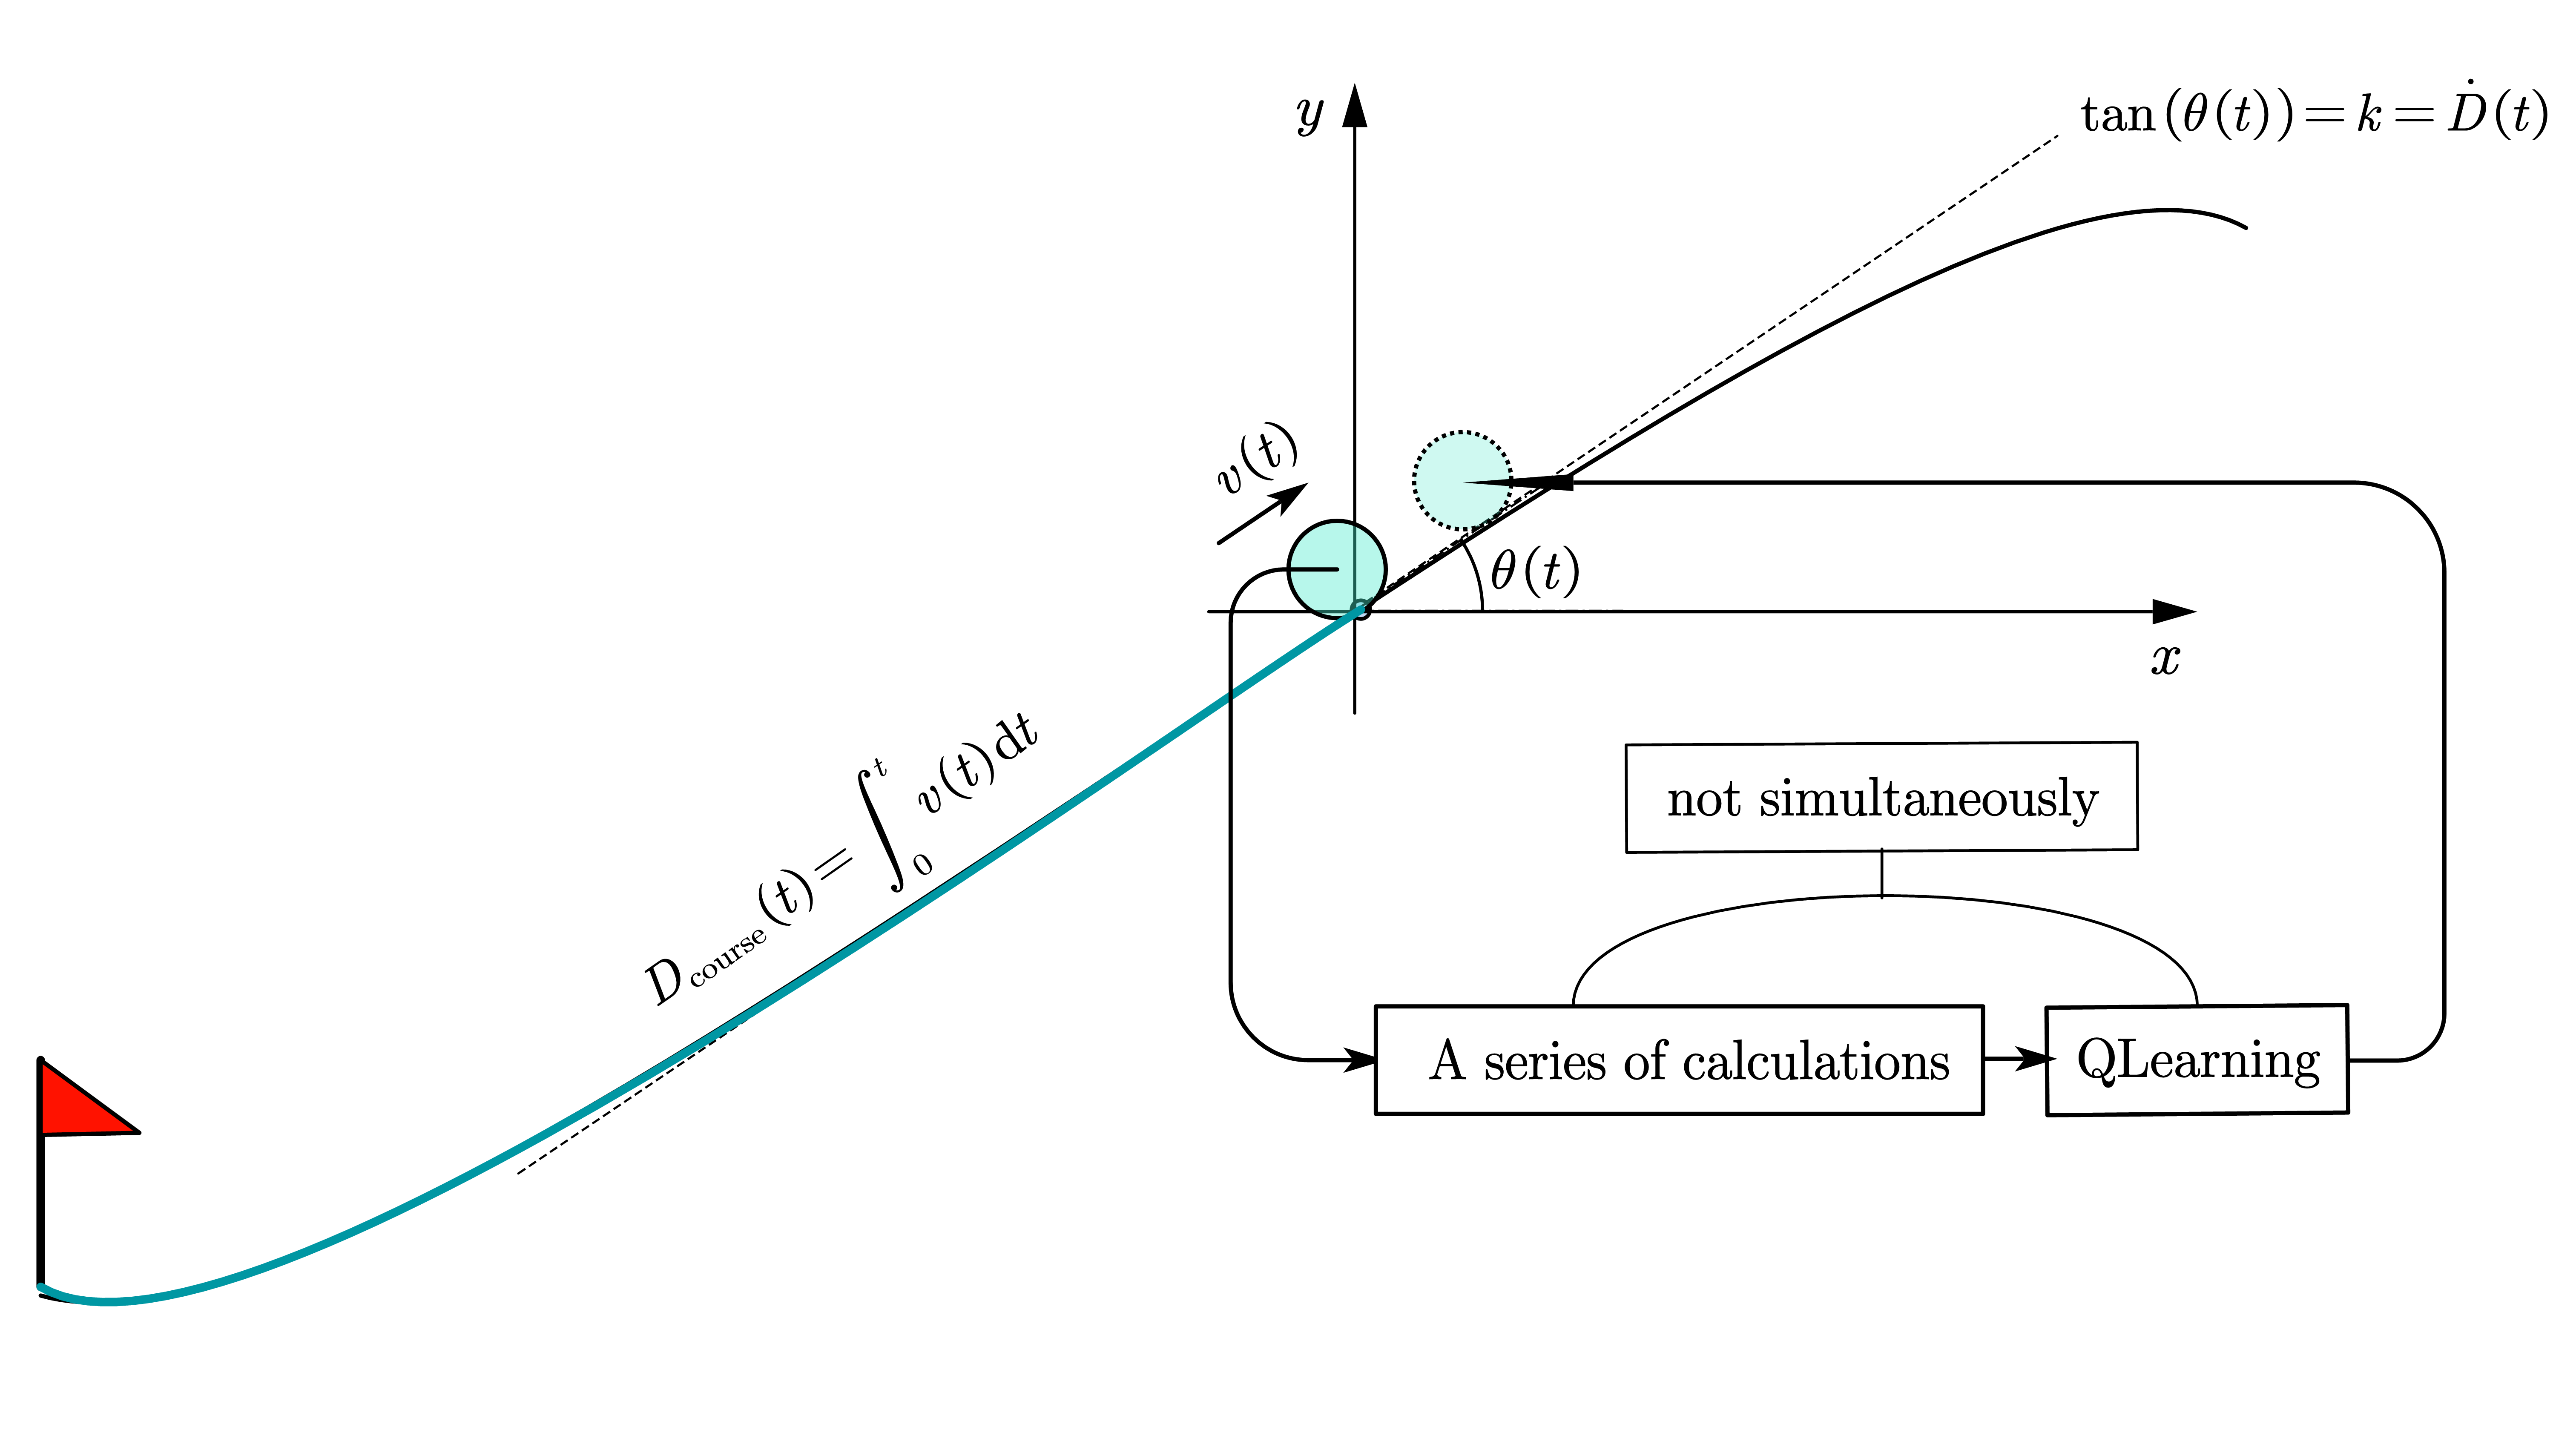
\includegraphics[height=8cm]{Recalculating speed function.png}

				\small\textit{Fig. Process of the algorithm}
			\end{center}

			Here, we also list the retationships between variables till now to show it more explicitly in the Q-learning process:\

			\begin{center}
				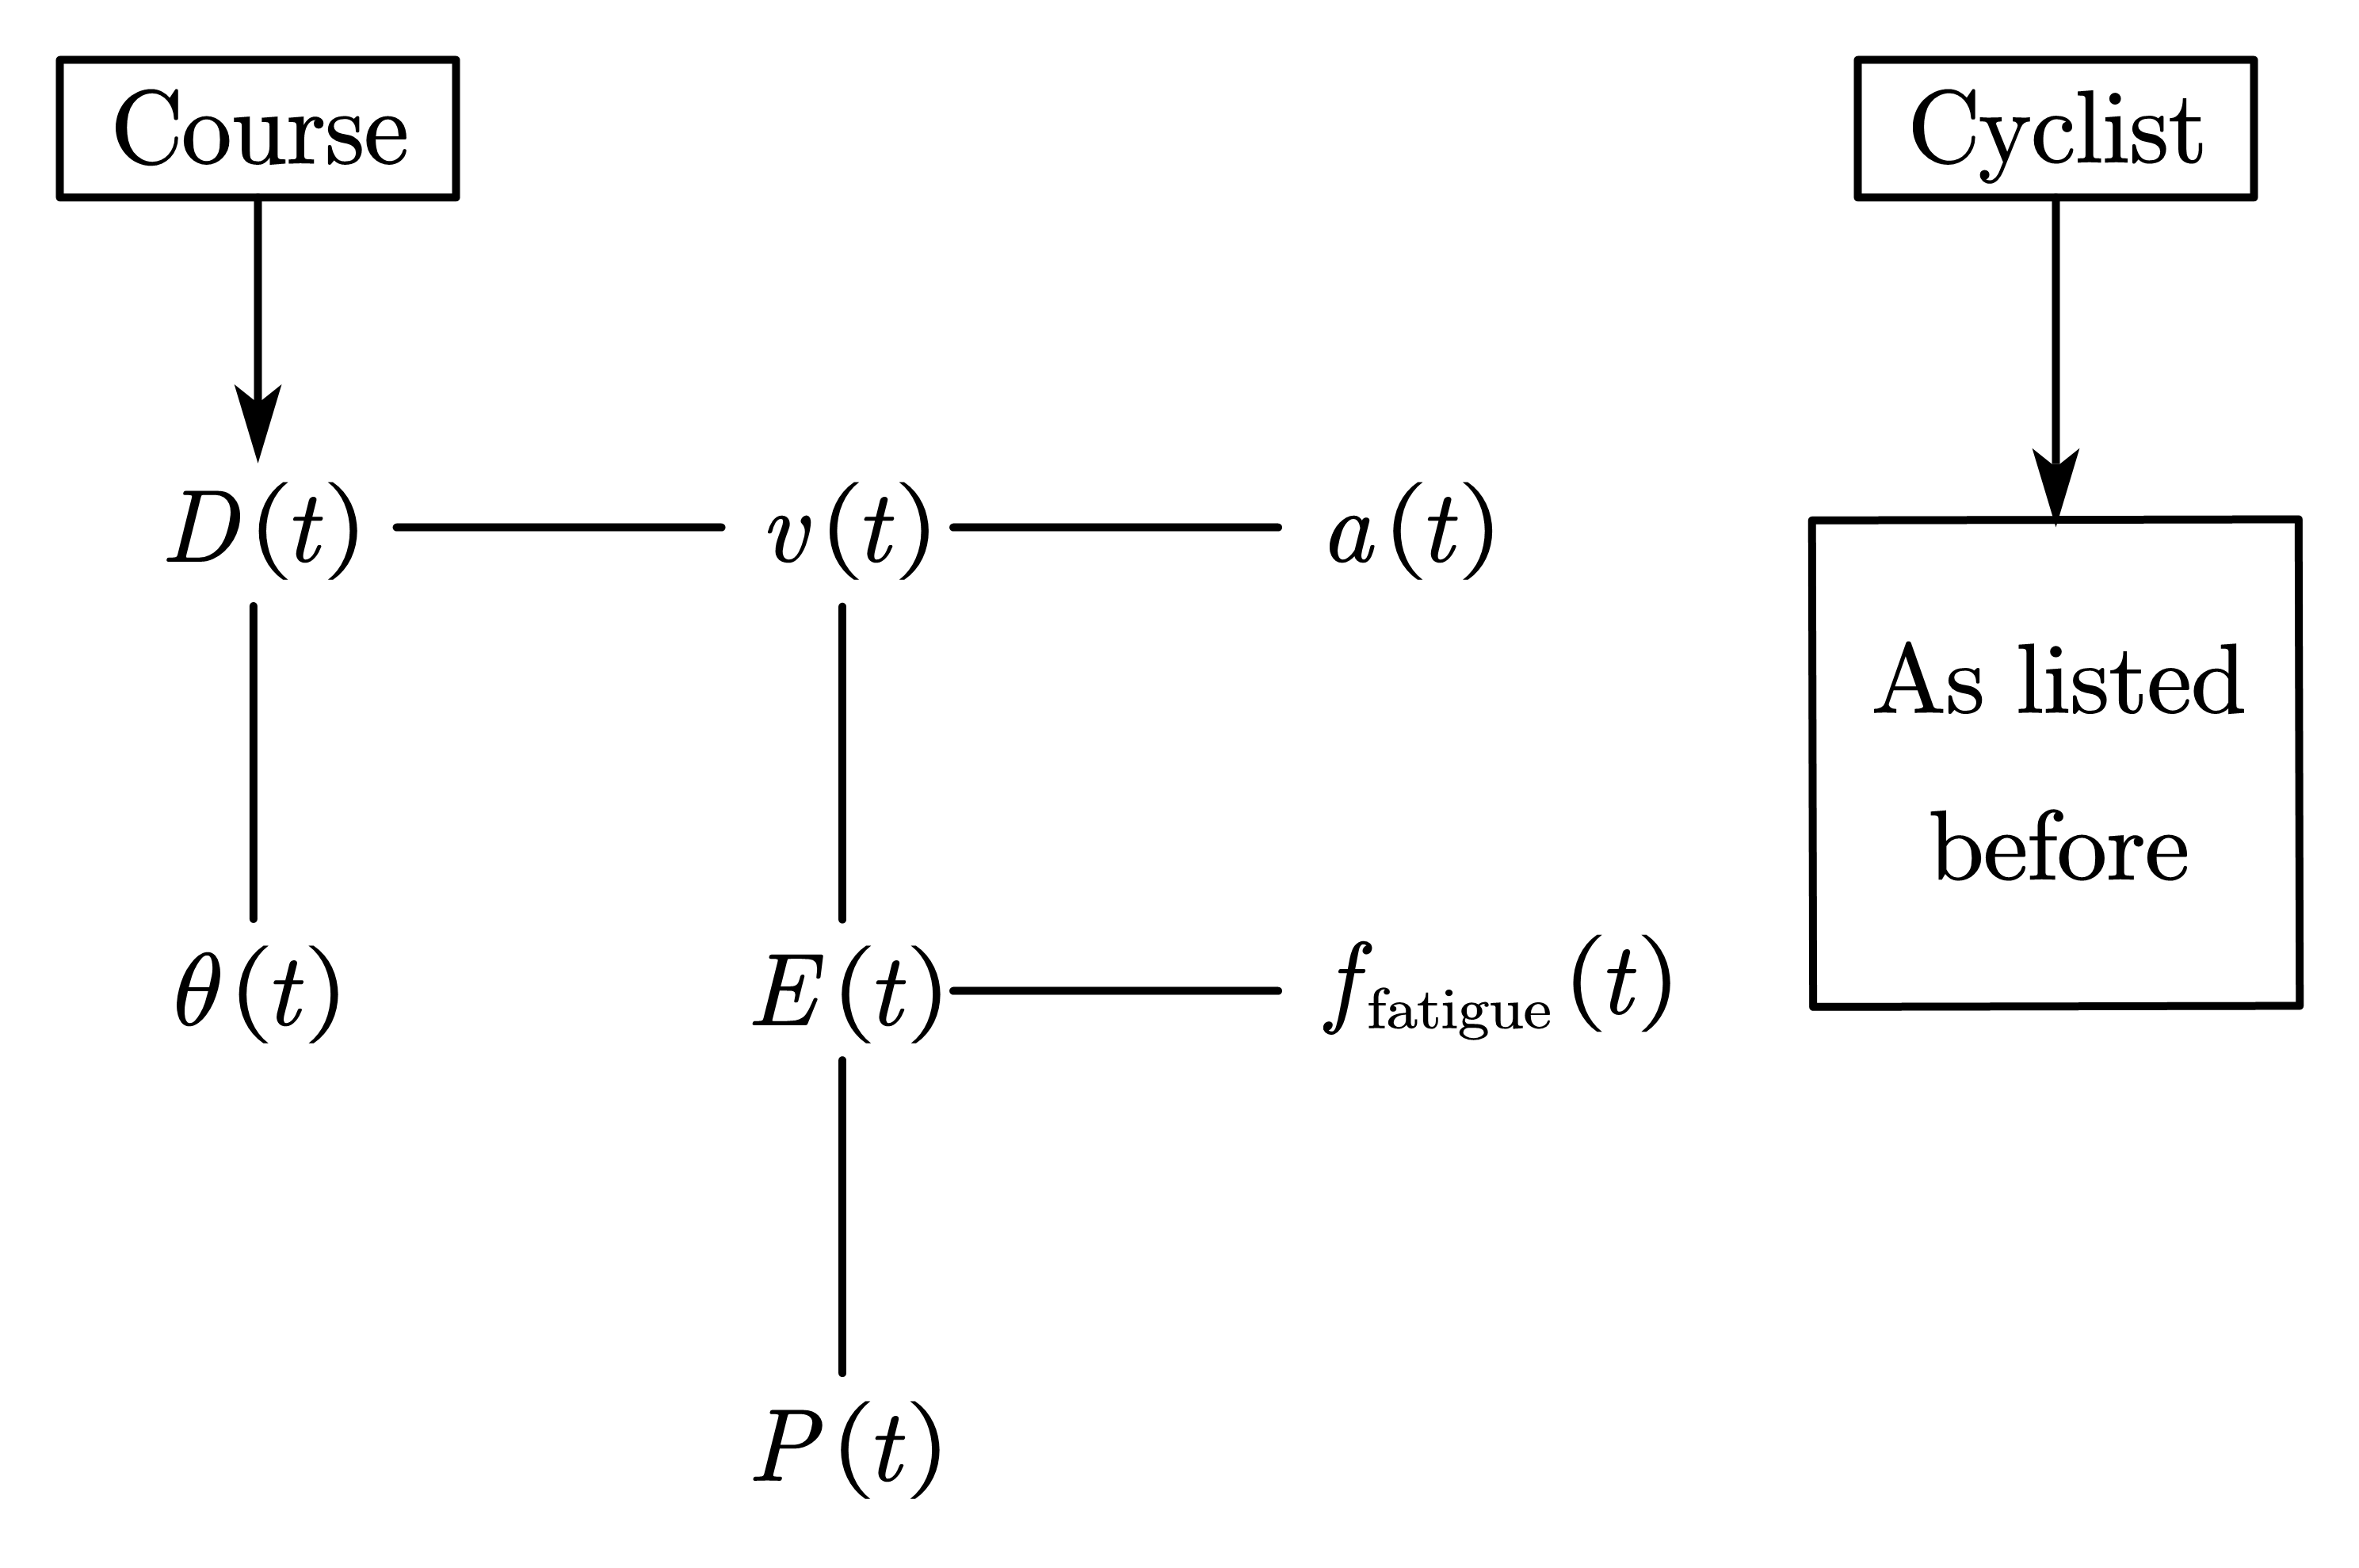
\includegraphics[height = 6cm]{the relationship between variables.png}

				\small\textit{Fig. The relationships between variables}
			\end{center}
		\subsection{The Q-Learning Algorithm}
			In this section, we'll mainly discuss the realization of the Q-Learning algorithm and its mechanism on different kinds of participants, which is also required by the problem.

			\subsubsection{Indicators related to the learning process}
				\begin{itemize}
					\item \textbf{The fatigue index \(f_{\mathrm{fatigue}}\)}

						Since our powercurve is a successive function, we define \(f_{\mathrm{fatigue}}\) as the \textit{fatigue index}. The higher \(f_{\mathrm{fatigue}}\) is, the more \textit{tired} he/she is. With a qualitative analysis, we can first find out the trend between \(f_{\mathrm{fatigue}}\) and other indicators \& variables:

						\[
							\begin{cases}
								E(t)\downarrow\Rightarrow f_{\mathrm{fatigue}}\uparrow \\
								\dfrac{\mathrm{d}}{\mathrm{d}t}E(t)\downarrow\Rightarrow f_{\mathrm{fatigue}}\uparrow
							\end{cases}
						\]
						(the second equation means that the more rapidly the cyclist is exhausting energy at time \(t\), the more exhausted he/she will be.)

						To be accurate, we define:
						\[
							\begin{aligned}
								f_{\mathrm{fatigue}}\left( t \right) &=\alpha _{\mathrm{fatigue}}\times \mathrm{energy}\:\:\mathrm{proportion}\times \mathrm{how}\:\:\mathrm{tired}\:\:\mathrm{you}\:\:\mathrm{are}
								\\
								&=\alpha _{\mathrm{fatigue}}\cdot \dfrac{E\left( t \right)}{E_{\mathrm{total}}}\cdot \left( \dfrac{\mathrm{instant}\:\:\mathrm{fatigue}\:\:\mathrm{rate}}{f_{\mathrm{fatigue}}^{\Theta}} \right) ^{-1}
								\\
								&=\alpha _{\mathrm{fatigue}}\cdot \dfrac{E\left( t \right)}{E_{\mathrm{total}}}\cdot \dfrac{E\left( t \right) -E_{\mathrm{total}}}{t\cdot \dot{E}\left( t \right)}
							\end{aligned}
						\]

						where:
						\[
							standard\:\:\mathrm{fatigue}\:\:\mathrm{rate}\left( f_{\mathrm{fatigue}}^{\Theta} \right) \xlongequal{\mathrm{def}}\mathrm{average}\:\:\mathrm{fatigue}\:\:\mathrm{rate}=\dfrac{E\left( t \right) -E_{\mathrm{total}}}{t}
						\]

						In addition, \(f_{\mathrm{fatigue}}\) also plays a decisive role in indicating the learning rate \(\alpha\) which we note here as \(L\) for brevity. We apply the commonplace \textit{S function} in statistics to our model, since the function appears to be swift-changing to the extremes and evenly-distributed in the middle. We plot this after a swift translation and stretching:
						\[L\left( f_{\mathrm{fatigue}} \right) =1-\underset{\mathrm{the}\:\:\mathrm{lower}\:\:\mathrm{bound}\:\:\mathrm{rate}}{\underbrace{\dfrac{2}{3}}}\sigma \left( \underset{\mathrm{the}\:\:\mathrm{stretching}\:\:\mathrm{rate}}{\underbrace{10}}\cdot \left( \underset{\mathrm{translation}}{\underbrace{\dfrac{1}{2}-x}} \right) \right) \]
						\begin{center}
							\includegraphics[height = 6cm]{the relationship between L and f_{fatigue}.png}

							\small\textit{Fig. the relationship between \(L\) and \(f_{\mathrm{fatigue}}\)}
						\end{center}
						We can plot this because previous equations have already indicated that \(\alpha _{\mathrm{fatigue}}\in \left[ 0,1 \right] \).
					\item \textbf{the Attribute Vector of an individual cyclist \(\vec{v}\)}

						Previously we've already listed the variables that change through time. We compile those into an \defword{attribute vector} for each individual cyclist \(\vec{v}=\left( v_1,v_2,...,v_k \right) \).

						Wherever the cyclist is on the route, due to the continuity of the functions, there is always an \textit{ideal} vector set of this specific point which we note as \(\vec{v}^{\Theta}=\left( v_{1}^{\Theta},v_{2}^{\Theta},...,v_{k}^{\Theta} \right)\).

						We define the \defword{gap} between the current vector state and the ideal vector state as:
						\[\Delta ^{\Theta}v=\sqrt{\dfrac{\displaystyle\sum\limits_{i=1}^k{\left( v_i-v_{i}^{\Theta} \right) ^2}}{k}}\xlongequal{\mathrm{def}}f_{\Delta}\left( \vec{v} \right) \]

						Therefore the maximum descent with this \(f_{\Delta}\left( \vec{v} \right)\) at point \(t\) equals \[\nabla f_{\Delta}\left( \vec{v} \right)\], where \(\nabla\) represents the gradient operator.
				\end{itemize}
			\subsubsection{Q-Learning}
				\begin{algorithm}
					\caption{Q-Learning}
					\begin{algorithmic}
						\STATE initialize Q-table
						\STATE initialize S
						\STATE $f_{\mathrm{fatigue}}\leftarrow 0$
						\FOR{ athlete $i$}
						\STATE randomly initialize the parameter vector $\vec{v}=\left( v_1,v_2,...,v_k \right)$ of $i$ \# showing his parameters
						\STATE his current strategy vector $\vec{v\left(t\right)}=\left( v_1\left(t\right),v_2\left(t\right),...,v_k\left(t\right) \right)$ \# showing his strategy
						\ENDFOR
						\WHILE{not at the ending point}
						\STATE \# change his strategy vector $\vec{v\left(t\right)}$ according to Q-table
						\STATE choose a strategy \textbf{$A$} based on $\vec{v\left(t\right)}$ and \textbf{P}
						\STATE calculate the expected (best) strategy for the current terrain based on previous calculations $\vec{v}^{\Theta}=\left( v_{1}^{\Theta},v_{2}^{\Theta},...,v_{k}^{\Theta} \right) $
						\STATE
						\STATE $\Delta ^{\Theta}v\leftarrow \sqrt{\dfrac{\sum\limits_{i=1}^k{\left( v_i-v_{i}^{\Theta} \right) ^2}}{k}}\xlongequal{\mathrm{def}}f_{\Delta}\left( \vec{v} \right) $
						\STATE
						\STATE $Q(S,A)\gets (1-\underset{\mathrm{learning}\:\:\mathrm{rate}}{\underbrace{\alpha }})Q(S,A)+\underset{\mathrm{learning}\:\:\mathrm{rate}}{\underbrace{\alpha }}[\underset{\mathrm{reward}}{\underbrace{R}}+\underset{\mathrm{discount}\:\:\mathrm{factor}}{\underbrace{\gamma }}\cdot \mathrm{inverse}\:\:\mathrm{strategy}\left( \nabla f_{\Delta}\left( \vec{v} \right) \right) -Q(S,A)]$
						\STATE
						\STATE \# learning rate $\alpha$ can change due to $f_{\mathrm{fatigue}}$
						\STATE \# when $f_{\mathrm{fatigue}}$ increases, $\alpha$ decreases
						\STATE Update Q-table
						\STATE Update $f_{\mathrm{fatigue}}$
						\STATE Update $\alpha$
						\ENDWHILE
						\STATE show the best strategy
					\end{algorithmic}
				\end{algorithm}


		\subsection{Applying to Real-life Trials}
		Now that we have figured out the power pattern of cyclists, we can apply it to trials and find out whether it is sensitive in real life. There are three trial courses in our model. The first is 2021 Olympic Time Trial course in Tokyo\cite{tokyo}, the second is 2021 UCI World Championship time trial course in Flanders\cite{UCI}. Both of the courses has the same features: they have at least one sharp turn and numerous gentle slopes.

		\begin{center}
			
\includegraphics[width=15cm]{6.png}\\
			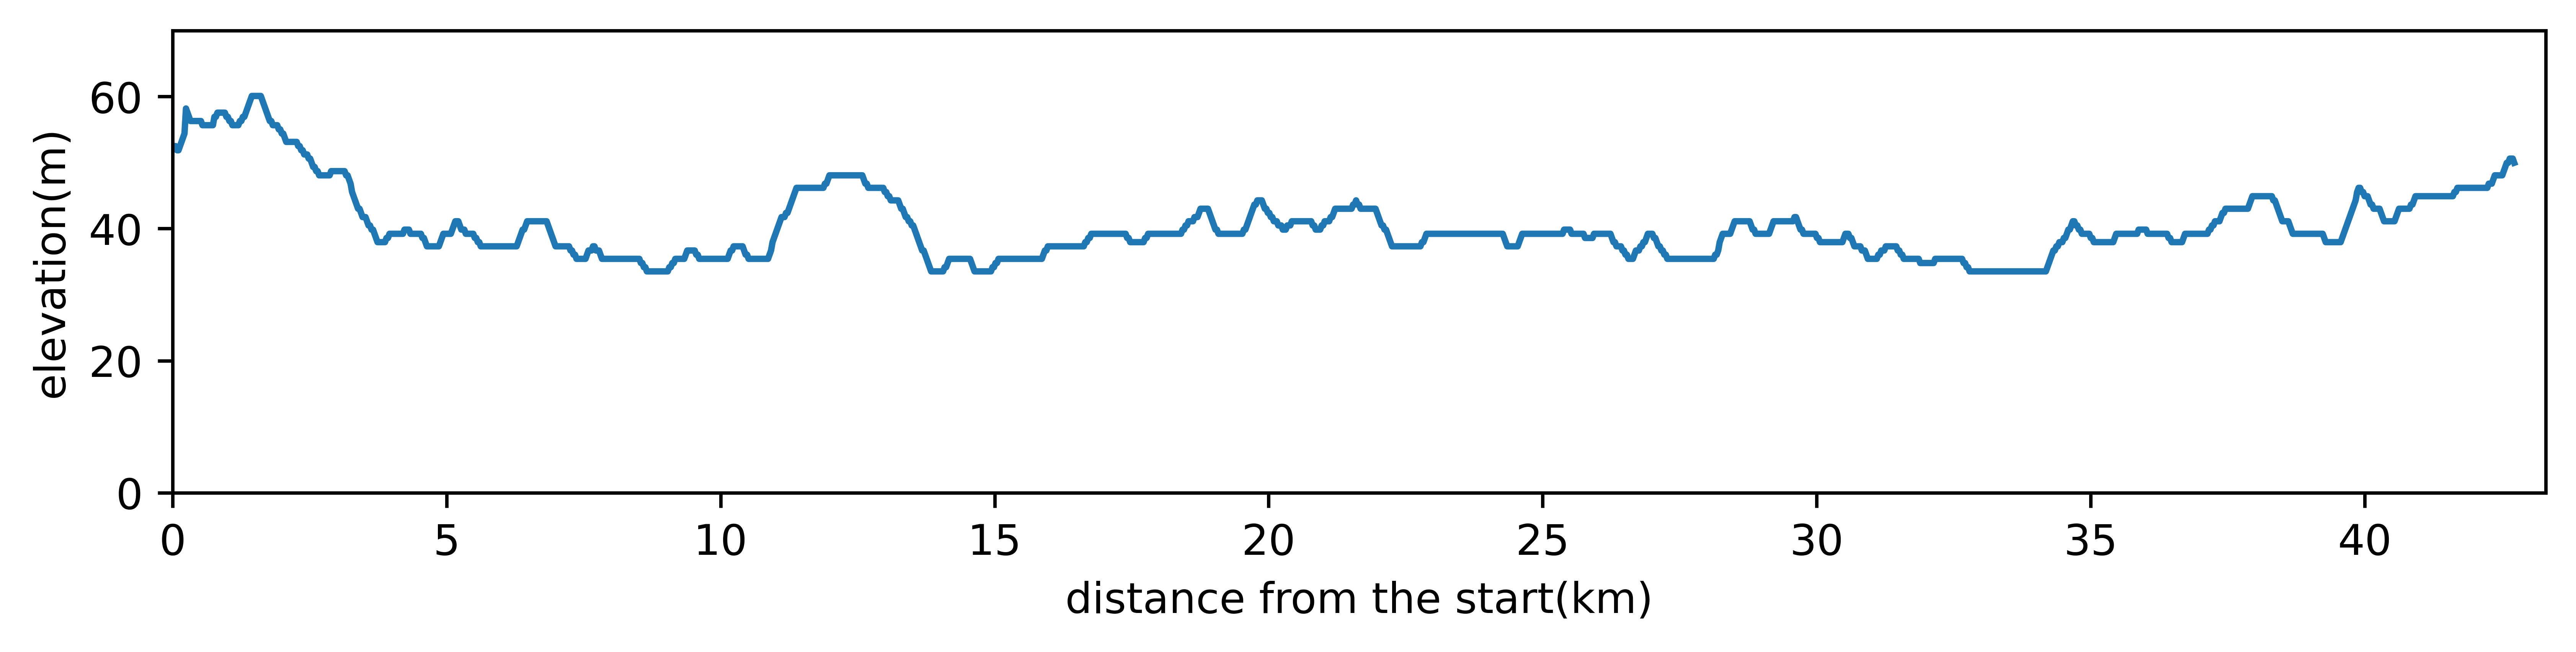
\includegraphics[width=15cm]{7.png}\\
			\small \textit{Fig. 6 and 7  Different trial courses}
		\end{center}

		As the curve of velocity to time is very complicated, it's difficult for us to calculate the precise value of the total time. However, according to the shape of the curve, some easier routes and the real data of athletes participating in the race, we can estimate that the average speed in this kind of race whose route is long and slope is gentle is approximately equal to two thirds of the maximum speed of bicycles.

		Under this hypothesis, the best possible score that can be achieved is around 36 minutes while the best performance in 2021 is around 46 minutes. Considering the exhaustion during the race, this result is rather reasonable.

		\subsection{Sensitivity Analysis}
			We are required to conduct a sensitivity analysis on variables which we note as \(\mathrm{Index}_i\) to the eventual power curve \(P(t)\). A universal version of the calculation originates from the idea of gradually doing the analysis from bottom up, which is written below (for those such as the meteorological parameters, the subsequent equations should be rendered depending on the specific case that they work on):
			\[
				\begin{aligned}
					S\left( P\left( t \right) ,\mathrm{Index}_i \right) &=\lim_{\Delta \mathrm{Index}_i\rightarrow 0} \dfrac{\dfrac{\Delta P\left( t \right)}{P\left( t \right)}}{\dfrac{\Delta \mathrm{Index}_i}{\mathrm{Index}_i}}=\lim\limits_{\substack{\Delta \mathrm{Index}_i\rightarrow 0 \\\Delta \mathrm{Rider}_i\rightarrow 0\\\Delta\Delta^{\Theta}v\rightarrow 0}} \left( \dfrac{\dfrac{\Delta \mathrm{Rider}_i}{\mathrm{Rider}_i}}{\dfrac{\Delta \mathrm{Index}_i}{\mathrm{Index}_i}}\cdot \dfrac{\dfrac{\Delta \Delta ^{\Theta}v}{\Delta ^{\Theta}v}}{\dfrac{\Delta \mathrm{Rider}_i}{\mathrm{Rider}_i}}\cdot \dfrac{\dfrac{\Delta P\left( t \right)}{P\left( t \right)}}{\dfrac{\Delta \Delta ^{\Theta}v}{\Delta ^{\Theta}v}} \right) \\
					&=S\left( P\left( t \right) ,\Delta ^{\Theta}v \right) \times S\left( \Delta ^{\Theta}v,\mathrm{Rider}_i \right) \times S\left( \mathrm{Rider}_i,\mathrm{Index}_i \right)
				\end{aligned}
			\]

			\subsubsection{Sensitivity of temperature}
				According to the \textit{layer-by-layer} analytical process and previous formulae, we have:
				\[
					\begin{aligned}
						S\left( P\left( t \right) ,\tau \right) &=S\left( \sigma ,\tau \right) \times S\left( P\left( t \right) ,\sigma \right) =S\left( \sigma ,\tau \right) \times S\left( \dot{E}\left( t \right) ,\sigma \right) \\
						&= \dfrac{E_{\mathrm{total}}\cdot e^{-\frac{E_{\mathrm{total}}}{K_b\tau}}}{K_b\tau ^2}\cdot \dfrac{\tau}{\sigma}=\dfrac{E_{\mathrm{total}}\cdot e^{-\frac{E_{\mathrm{total}}}{K_b\tau}}}{K_b\tau ^2}\cdot \dfrac{\tau}{e^{-\frac{E_{\mathrm{total}}}{K_b\tau}}}=\dfrac{E_{\mathrm{total}}}{K_b}\cdot \tau ^{-1}
					\end{aligned}
				\]
				We plot it below:
				\begin{center}
					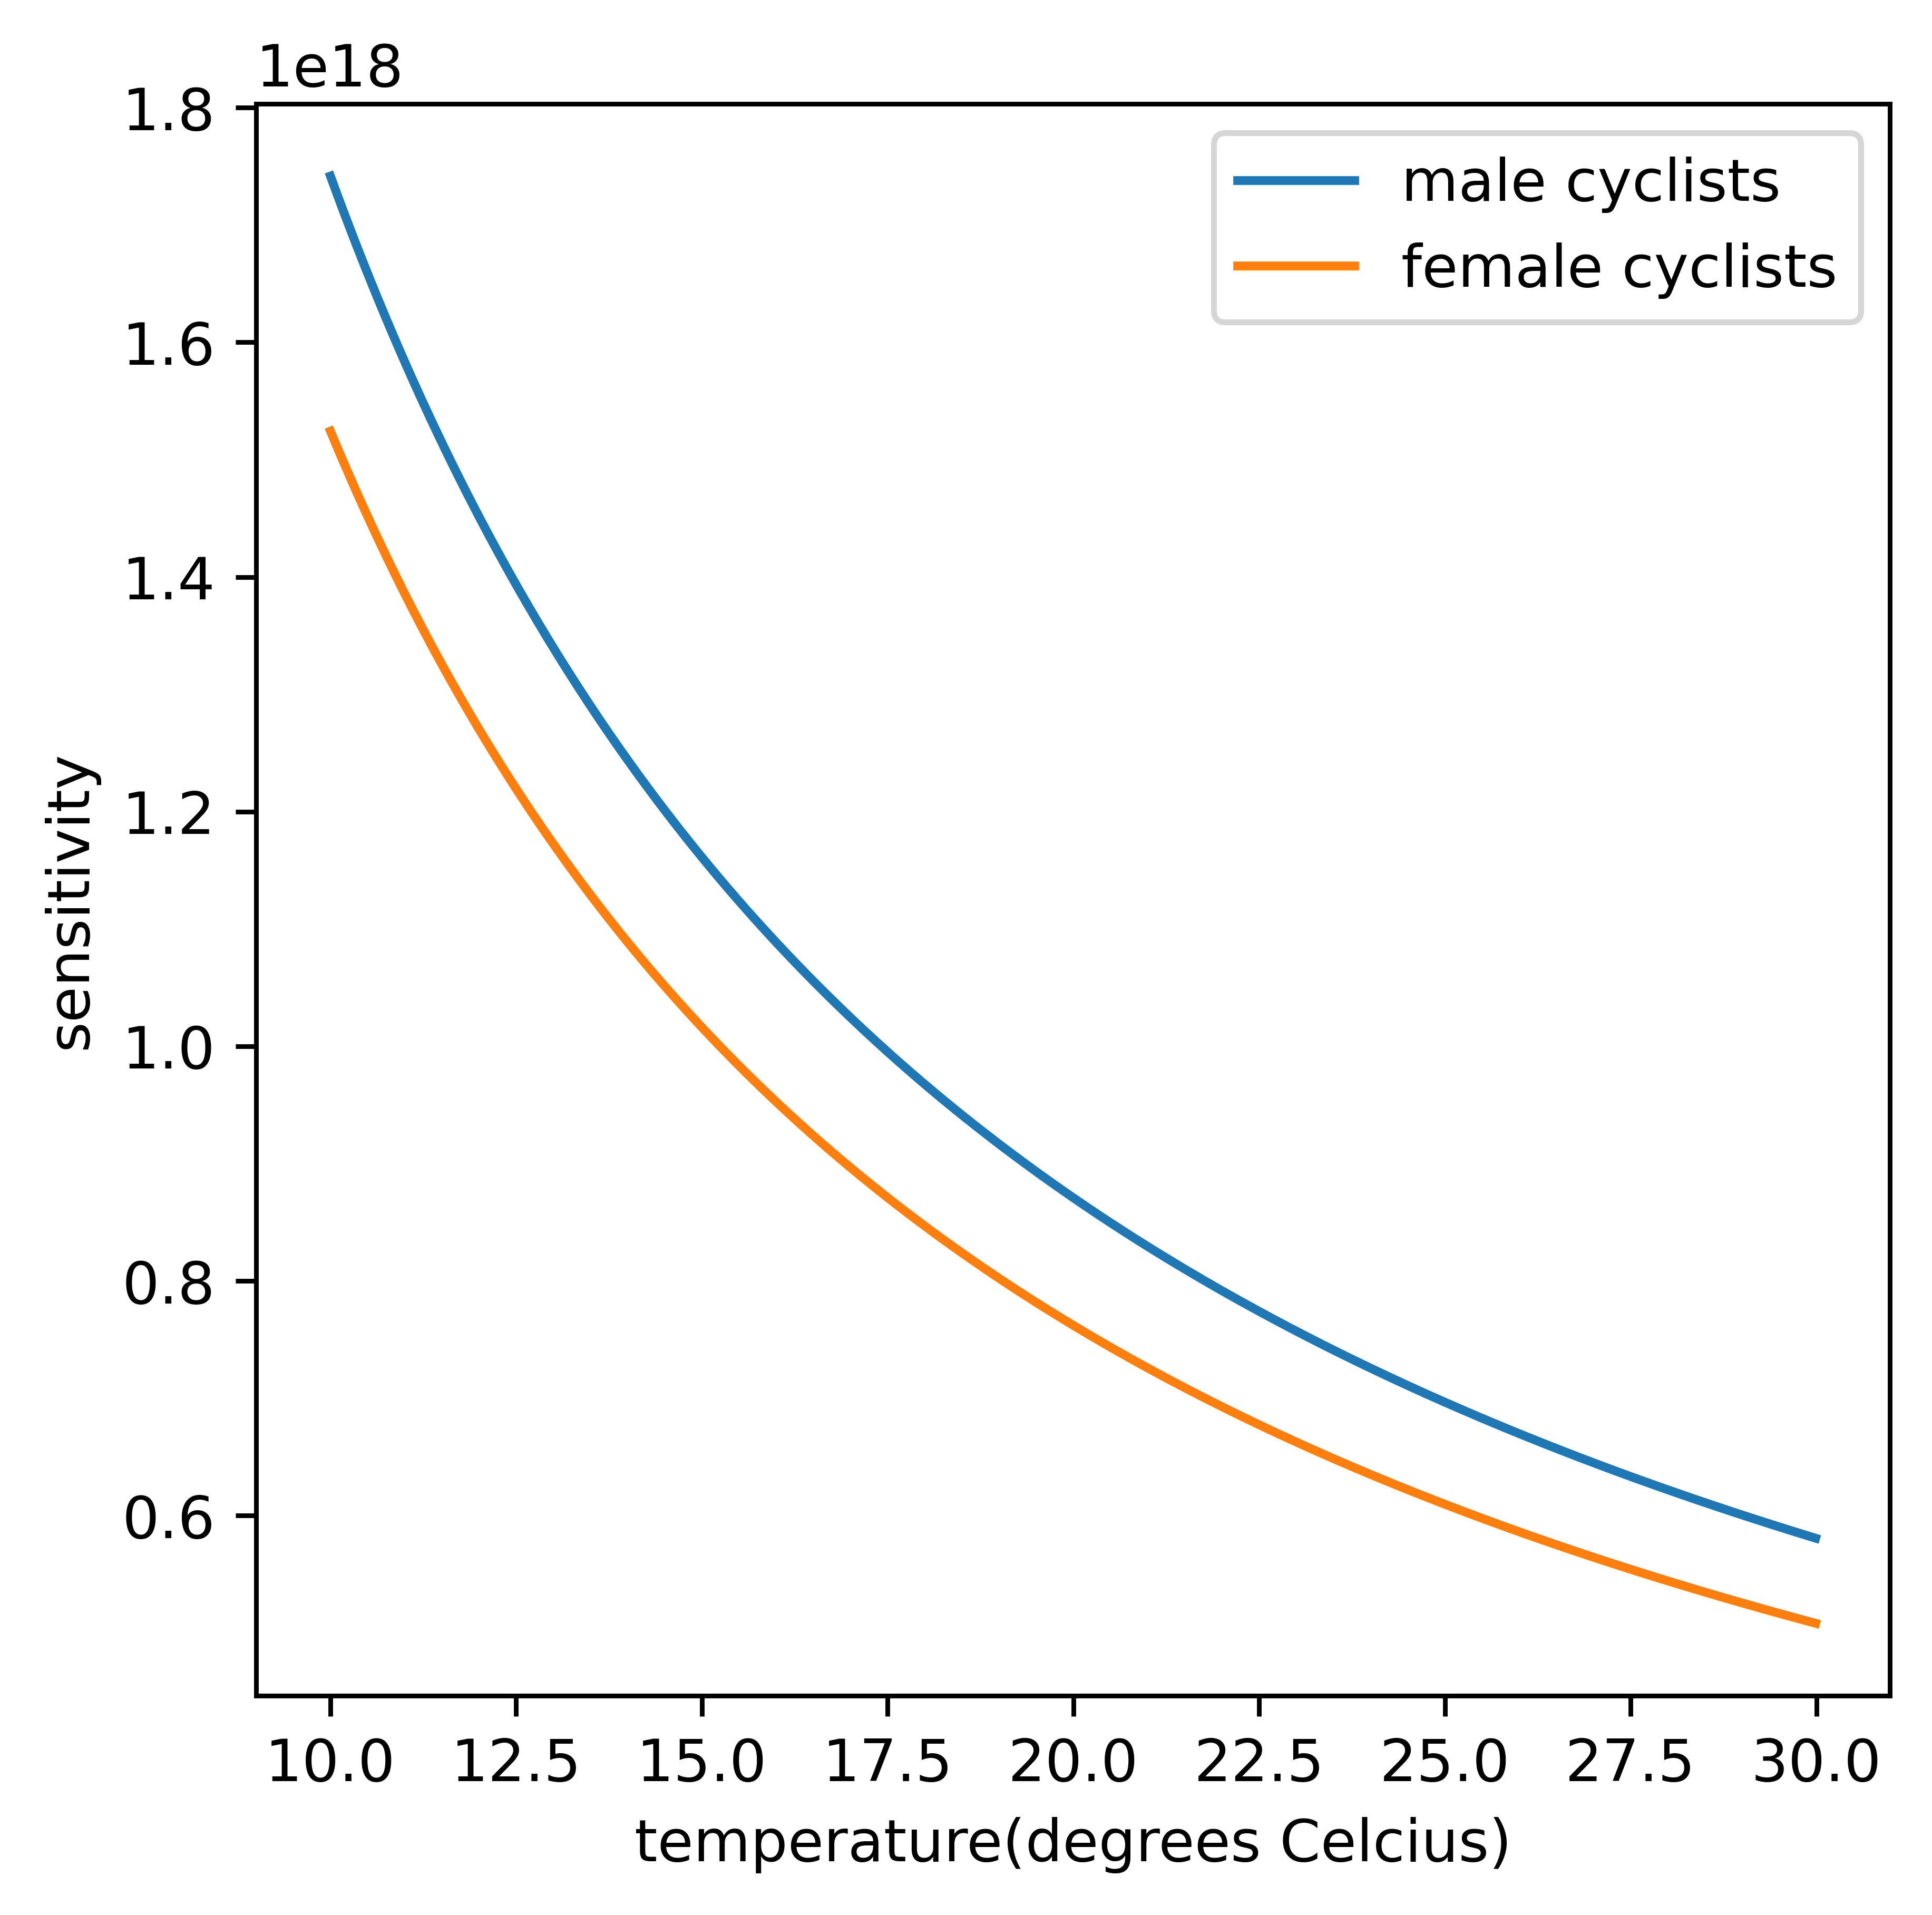
\includegraphics[height = 6cm]{sensitivity analysis of temperature.png}

					\small\textit{Fig. Sensitivity analysis of temperature}
				\end{center}
				We find that power curve is rather sensitive to the variations in temperature.
			\subsubsection{Sensitivity of wind strength}
				We conduct similar procedures on wind force:
				\[
					S\left( P\left( t \right) ,F_{\mathrm{wind}} \right) =S\left( \dot{v}\left( t \right) ,F_{\mathrm{wind}} \right) \times S\left( \dot{E}\left( t \right) ,\dot{v}\left( t \right) \right)
				\]
				Calculate the sensitivity for each term, we get:\
				\[
					\begin{aligned}
						\dot{v}\left( t \right) &=\dfrac{P\left( t \right)}{mv}-g\sin \theta -\dfrac{k_{\mathrm{air}}}{2m}\left( v+v_{\mathrm{air}} \right) ^2
						\\
						&=\left( \dfrac{P\left( t \right)}{mv}-g\sin \theta -\dfrac{k_{\mathrm{air}}}{2m}v^2 \right) -\dfrac{k_{\mathrm{air}}}{2m\left( \rho _{\mathrm{air}}\cdot S_{\mathrm{body}} \right) ^2}F_{\mathrm{wind}}^{2}-\frac{k_{\mathrm{air}}}{m\cdot \rho _{\mathrm{air}}\cdot S_{\mathrm{body}}}F_{\mathrm{wind}}
					\end{aligned}
				\]
				We now estimate the coefficient of each term, which approximately equals \(6.5\times 10^{-4}\) for the derivative of the righ hand side (We can also get that there exists a linear relationship between the sensitivity). Therefore, we reach the conclusion that our model is far less sensitive on wind strength.












	\section{Model C}
		\subsection{Model Overview}
			After we built a dynamic model to simulate the cyclist's moving pattern, we extend our model to find out the best strategy for a team which is made up of 6 riders. We rank the cyclists according to their phisycal conditions ($E_\mathrm{total}$) and list out their "power cost" and determine thir "benefit" when different poeple lead the team. Finally, we will design several strategies and compare them with each other to find out the best solution.
		\subsection{Notation}
			\begin{tabular}{|l|l|l|}
				\hline
				\(\left\{ a_i \right\} _{i=1}^{6}\) & the 6 participants ranked from the most to least capable &/ \\
				\hline
				\(\bar{P\left( t \right) }\) & the Power curve of \(a_4\) & continuous function \\
				\hline
				\(s_i\) & the \(i^{\mathrm{th}}\) state of the fleet & \(3\times 2\) matrix \\
				\hline
				\(\tau\) & the points of time during an exchange & \(\mathrm{s}\)\\
				\hline
				$v(P_\mathrm{decline})$&declining speed of power& continuous function\\
				\hline
				$P_\mathrm{cost}$&the criteria power of the fleet& continuous function\\
				\hline
				$P_\mathrm{benefit}$&gap between the power of the leader and the criteria power& continuous function\\
				\hline
			\end{tabular}
		\subsection{Ranking the Cyclists}
			First we need to rank the cyclists based on their strength. In our model, the most intuitive way to rank them is to find out their total energy ($E_\mathrm{total}$) since it's related to the cyclist's physical condition. We rank their $E_\mathrm{total}$ and rename them from $a_1$ to $a_6$. Since the team's time is determined when the fourth rider crosses the finish line. We take the power curve of $a_4$ as the criteria, which we call "power cost". Therefore, we can compare the "benefit power" of this team when a different cyclist is leading the fleet.
			\begin{center}
				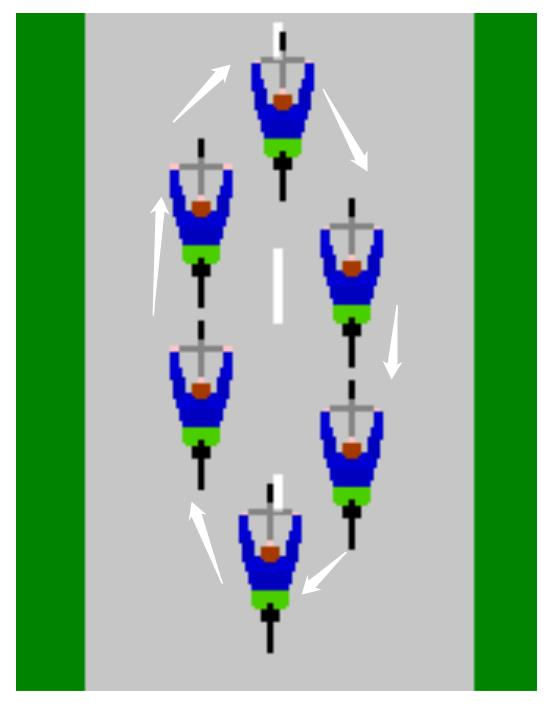
\includegraphics[height = 4cm]{clockwise.jpg}
				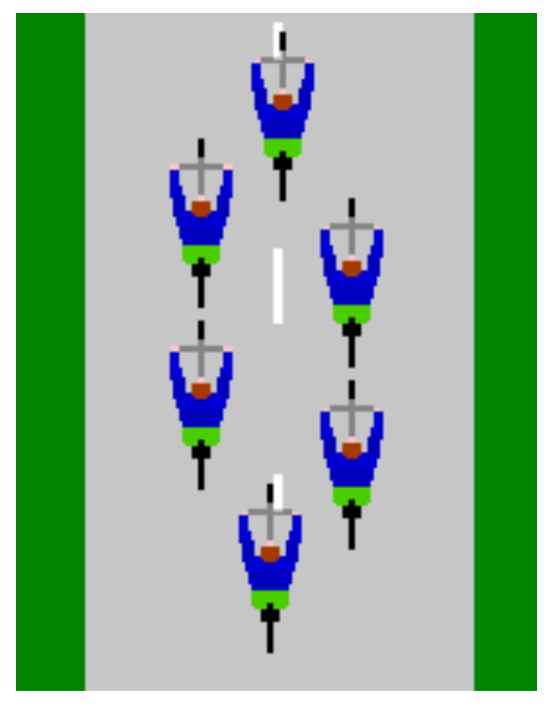
\includegraphics[height = 4cm]{fleet actions.png}
				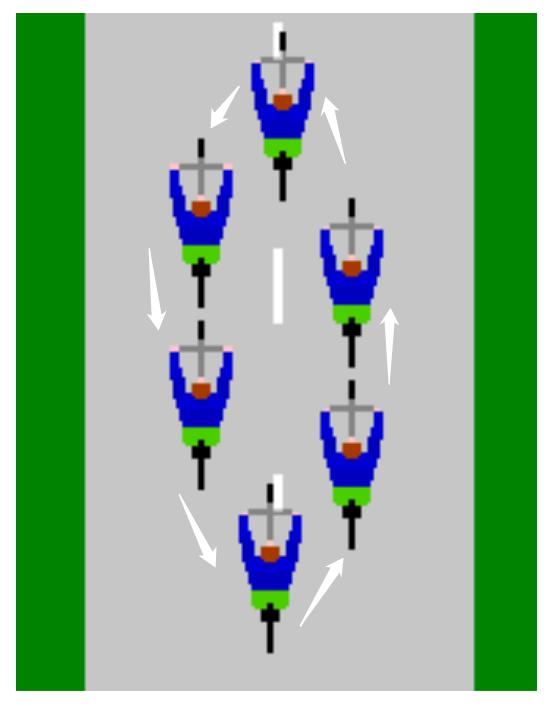
\includegraphics[height = 4cm]{counterclockwise.jpg}

				\small\textit{Fig. simulation of the fleet exchange action}
			\end{center}
				We define \(T^{\left( \circlearrowleft \right)}\) as a counterclockwise change in the fleet, and \(T^{\left( \circlearrowright \right)}\) as a clockwise one. Suppose the \(i^{\mathrm{th}}\) exchange starts at \(\tau_{1,T_i}\) and ends at \(\tau_{2,T_i}\). To simplify mathematical calculations, we abstract the whole fleet into a \(3\times 2\) matrix:

				\[s_i=\left[ \begin{matrix}
					a_{11}&		a_{12}\\
					a_{21}&		a_{22}\\
					a_{31}&		a_{32}\\
				\end{matrix} \right] \]
				, where \(a_{11}\) leads the team and \(a_{32}\) behind it.

				We use \(r\left( a_{ij} \right) \) to give the ranking of element \(a_{ij}\) in \(s_i\). Notice that a cyclist with energy below \(\bar{P\left( t \right) }\) draws back the team's overall performance while the other conversely. We define the \defword{benefit} of an exchange process as:

				\[P_\mathrm{benefit} =\int_{\tau _{1,T_i}}^{\tau _{2,T_i}}{\left( P_{\mathrm{new}\:\:\mathrm{comer}}\left( t \right) -P_{\mathrm{avg}}\left( t \right) \right)}\], which can be positive or negative. For those with positive \defword{benefits}, the maximum of the integral takes place when \(P_{\mathrm{new}\:\:\mathrm{comer}}\left( t \right) -P_{\mathrm{avg}}\left( t \right) =0\).

				Next, we need to find out the velocity change when there is "leader change". When a cyclist becomes the leader, his body is fully exposed to the air and needs to endure all the air resistance (wind force) caused by the environment. Using the energy to deal with these bothering factors, his power will decline at a higher speed. On the other hand, when a cyclist rides after the leader, some part of his body was covered by the leader. This means that he was slightly affected by the air, giving him the chance to recover. Therefore there is a obvious differnce between their $v(P_\mathrm{decline})$. Or in other words:

				\[
					\begin{cases}
						\dfrac{\mathrm{d}}{\mathrm{d}t}P_{a_{11}}\left( t \right) \propto \dfrac{\mathrm{d}}{\mathrm{d}t}P_{\mathrm{others}}\left( t \right)\\
						f_{\mathrm{air}\:\:\mathrm{others}}=0\\
					\end{cases}
				\]



	\section{Strengths and Weaknesses}
		\subsection*{Strengths}
			\begin{itemize}
				\item\textbf{Accuracy}

					As relevant constants that appear in our models are not always accessible on the Internet, we adopted the method of fitting data into our model, which derived rather reasonable results. We build a dynamic model to speculate on the cyclist's moving pattern, velocity condition and energy consumption. These two combined, therefore, actually results in a even more accurate model with computational convenience, accuracy and reality.
				\item\textbf{Generality}

					Another part of our model with deep insight is that, instead of attempting to establish a universal model which is able to effectively cope with all types of scenarios, we developed two models (Model A \& B) which respectively excels in patterns with regular slopes and those with irregular ones.
				\item\textbf{Just a Single Data}

					In our model, we use only single type of data. This means that we only need a little time to collect the data needed in our model and athletes don't have to worry about providing a variety of data.
			\end{itemize}
		\subsection*{Weaknesses}

			\begin{itemize}
				\item\textbf{Complexity}

					In the second model, we use large amount of calculus to make our calculations more accurate. This make our model more complex. It need more time to run and more difficult to understand, which is not convenient for us to explain it to cyclists.
				\item\textbf{Not Concerning Kinematic Law}

					To simplify our calculations, we only take the cyclist's energy consumption into consideration when it comes to team strategies. However, our calculations may not obey the kinematic law. As a result, there is chance that our calculations are contrary to reality.

			\end{itemize}
	\newpage
	\section{Rider's Guidance}
	\violetbf{Welcome to the 2021 Tokyo Olympic Time Trial guidance for participants.} This is \textcolor{purple}{MCM Mathematical Modeling Group}. To facilitate you achieve the best score, we have built a dynamic model to give you basic instructions at different stages based on your physical conditions and your riding habits. \violetbf{Now let's begin!}
	\begin{itemize}
	\itembf {Before the Race}

			Before the race, please hand us the cyclist's basic information including your age, gender, height, weight and which type of cyclist you are through email. This can help us be aware of your power and give you more detailed suggestions in the next phase. In addition, you need to know the whole trial course. This race is set up near the Fuji Mountain, and here's the map.\cite{tokyo}

			\begin{center}
				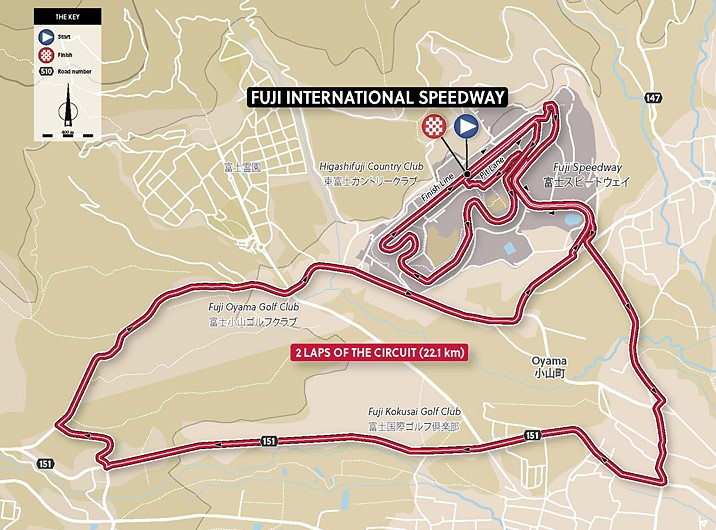
\includegraphics[width=9cm]{1.jpg}\\
				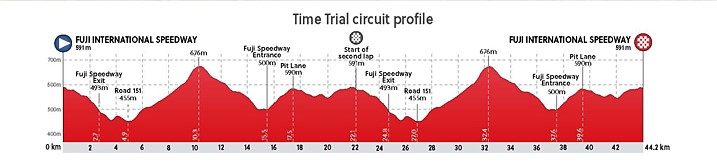
\includegraphics[width=14cm]{3.jpg}
			\end{center}

			Finally, you should keep a balanced diet and prepare enough energy supplement before the race. We will introduce it to you in the next section.
	\itembf{During the Race}
	\begin{enumerate}
		\itembf{Put on Heat-Preserving Clothes}

			According to our research, temperature has an outsize effect on a cyclist's power consumption speed. To make sure that you won't be quickly exhausted due to temperature decline, you should wear warm clothes or bring some thermal insulation devices with you.
	\end{enumerate}
	\end{itemize}
	That's the end of this guidance. If your have any questions during reading, please send us an email or dial us.\violetbf{Hope you enjoy yourself during the race and achieve the best score!}

	Yous sincerely,
	\textcolor{purple}{\textbf{MCM Math Modeling Group}}
	\newpage
	\section{Letter To the Two Athletes}
	\newpage
	\thispagestyle{empty}
	% \setcounter{page}{\wholepages}
	\renewcommand\refname{References}
	\clearpage
	\addcontentsline{toc}{section}{References}
	\tolerance=500
	\begin{thebibliography}{100}
		\bibitem{114514} Mathematical Modelling, Qiyuan Kang, Jinxing Xie and Jun Ye
		\bibitem{UCI}2021 Road World Championships Individual Time Trial (Men Elite), UCI,

		https://www.flanders2021.com/\_media/races/image\_map/1632122636/fit/1650/0/6/men-elite-individual-time-trial.webp
		\bibitem{france}https://www.topendsports.com/sport/cycling/anthropometry-tourdefrance-tables.htm
		\bibitem{weight}Cycling Physique, science4performance,

		https://science4performance.com/2019/09/12/cycling-physique/
		\bibitem{friction}https://zhidao.baidu.com/question/309300297713546924.html
		\bibitem{boltzmann}Boltzmann constant, Dictionaty.com,

		https://www.dictionary.com/browse/boltzmann-constant/
		\bibitem{time trial record}The time trial speed record, en.wikipedia.org,

		https://en.wikipedia.org/wiki/List\_of\_cycling\_records/
		\bibitem{energy curve}Physical Strength Through Aging: What’s the Metric?, https://efficientexercise.com/

		https://efficientexercise.com/physical-strength-aging-whats-metric/
		\bibitem{time trial strategy}Team time trial, en.wikipedia.org

		https://en.wikipedia.org/wiki/Team\_time\_trial
		\bibitem {Qlearning} Simple Reinforcement Learning: Q-learning, Andre Violante,

		 https://towardsdatascience.com/simple-reinforcement-learning-Q-learning-fcddc4b6fe56
		\bibitem {tokyo} 2021 Olympic Time Trial for Men,UCI

		https://www.cyclingnews.com/races/olympic-games-2021/men-s-individual-time-trial/preview/
	\end{thebibliography}

\end{document}






